\documentclass[11pt,letterpaper]{article}

\usepackage[spanish,es-tabla]{babel}
\usepackage[utf8]{inputenc}
\usepackage[T1]{fontenc}
\usepackage{lmodern}
\usepackage{geometry}
\usepackage{microtype}
\usepackage{setspace}
\usepackage{amsmath,amssymb}
\usepackage{booktabs}
\usepackage{longtable}
\usepackage{array}
\usepackage{tabularx}
\usepackage{makecell}
\usepackage{multirow}
\usepackage{graphicx}
\usepackage{float}
\usepackage{adjustbox}
\usepackage{enumitem}
\usepackage{csquotes}
\usepackage[round,authoryear]{natbib}
\usepackage[colorlinks=true,linkcolor=blue,citecolor=blue,urlcolor=blue]{hyperref}
\usepackage[nameinlink,noabbrev]{cleveref}
\usepackage[section]{placeins}
\usepackage{caption}
\usepackage{subcaption}
\usepackage{pdflscape}
\usepackage{algorithm}
\usepackage{algpseudocode}

\geometry{margin=1in}
\onehalfspacing
\setlength{\parindent}{0pt}
\setlength{\parskip}{0.45em}
\setlist[itemize]{topsep=0.25em,itemsep=0.25em}
\setlist[enumerate]{topsep=0.25em,itemsep=0.25em}
\captionsetup{font=small,labelfont=bf}
\graphicspath{{figures/}}

\newcommand{\code}[1]{\texttt{\detokenize{#1}}}
\newcommand{\baselinepkg}{\code{mahoraga14_3_baseline}}
\newcommand{\officiallabel}{\code{MAHORAGA14_3_BASELINE_OFFICIAL}}
\newcommand{\officialcandidate}{\code{B1.05_C1.10_L1.10_R1.05}}
\newcommand{\historicalcontrol}{\code{MAHORAGA14_1_LONG_ONLY_CONTROL}}
\newcommand{\primaryvariant}{\code{MAHORAGA14_3_LONG_PARTICIPATION}}
\newcommand{\controlvariant}{\code{CONTINUATION_PRESSURE_V2_ONLY}}
\newcommand{\basealpha}{\code{BASE_ALPHA_V2}}
\newcommand{\allocator}{\code{PARTICIPATION_ALLOCATOR_V2}}
\newcommand{\conviction}{\code{CONVICTION_AMPLIFIER_LAYER}}
\newcommand{\leaderlayer}{\code{LEADER_PARTICIPATION_LAYER}}
\newcommand{\backoff}{\code{RISK_BACKOFF_LAYER_V2}}

\title{\textbf{Mahoraga como sistema quant general}\\
\large Arquitectura, logica operativa y auditoria del baseline oficial long-only congelado}
\author{Documento tecnico reproducible basado en el baseline oficial del repositorio QuantMahoraga}
\date{4 de mayo de 2026}

\begin{document}
\maketitle
\tableofcontents
\clearpage

\begin{abstract}
Este documento describe Mahoraga como sistema cuantitativo general y toma como culminacion operativa el baseline institucional congelado \officiallabel, publicado en el paquete \baselinepkg. El objetivo no es presentar una narrativa promocional ni reducir el proyecto a una comparacion aislada de rentabilidades, sino reconstruir de forma verificable que hace el sistema, que datos usa, como transforma informacion en decisiones, como asigna capital, que reglas limitan su conducta y como se audita formalmente.

El paper separa con rigor cuatro niveles que en proyectos cuantitativos suelen confundirse: (i) la arquitectura conceptual del sistema, (ii) los componentes efectivamente implementados en la ruta oficial, (iii) la historia de investigacion que llevo al baseline final y (iv) las intuiciones conceptuales que inspiraron parte del diseno pero no quedaron como modulos operativos. Esta distincion es especialmente importante en Mahoraga porque el baseline oficial no es una rama abierta de descubrimiento, sino una congelacion institucional de una arquitectura long-only promovida desde la familia 14.3R con cuatro multiplicadores aceptados localmente.

En terminos operativos, Mahoraga combina un nucleo de seleccion de acciones long-only basado en tendencia, momentum y residualizacion multifactor con una capa semanal de lectura de estado del mercado y del libro propio. Esa segunda capa no inventa alpha de seleccion; traduce evidencia de continuidad, amplitud, fragilidad, liderazgo y deterioro estructural en presupuesto de participacion, caps de exposicion, mezclas hacia lideres y mecanismos de backoff. El baseline publicado usa modelos de regresion logistica y un challenger de random forest en partes concretas del filtro temporal, pero no descansa en aprendizaje profundo, reinforcement learning ni IA generativa.

El documento tambien explica la metodologia de validacion: walk-forward, stitched OOS, ventanas prioritarias, leave-one-window-out, bootstrap por bloques estacionarios y una guarda de seleccion estilo reality-check sobre la familia local de candidatos. Los resultados oficiales reportados se toman exclusivamente de los outputs y auditorias congelados del repositorio. El stitched oficial del baseline presenta CAGR de 32.5518\%, Sharpe de 1.4826, Sortino de 2.5280 y MaxDD de -16.1997\%; sin embargo, este paper insiste en que esos numeros deben leerse junto con sus restricciones metodologicas, especialmente sesgo de supervivencia residual, dependencia de un universo concentrado y el hecho de que la promocion se defiende como punto robusto de una meseta local, no como optimo global probado.
\end{abstract}

\section{Introduccion}
Mahoraga es un proyecto cuantitativo que, en su estado oficial actual, debe entenderse como un \emph{sistema} y no como una formula unica. El baseline congelado del repositorio declara explicitamente que el modelo oficial es \officiallabel, congelado desde la referencia \code{Mahoraga14_3R / ROBUST_MAIN / B1.05_C1.10_L1.10_R1.05}, y destinado a servir como reemplazo institucional del control long-only previo \historicalcontrol \citep{quantBaselineDocs2026,quantGovernance2026}. Esta formulacion ya sugiere tres hechos importantes:

\begin{itemize}
    \item el baseline oficial es long-only;
    \item el baseline oficial es una congelacion gobernada, no una rama abierta de experimentacion;
    \item la unidad de analisis correcta no es un unico clasificador o una unica senal, sino una arquitectura con capas.
\end{itemize}

La pregunta central de este paper es, por tanto, la siguiente: \emph{como funciona Mahoraga, de extremo a extremo, en la version que el repositorio reconoce como baseline oficial?}

Responder esa pregunta exige ir mas alla del resultado stitched final. Hace falta distinguir entre el nucleo de seleccion de nombres, las capas de participacion alcista, los mecanismos de defensa, la logica de exposicion, la ruta de backtesting, los artefactos de auditoria y el proceso institucional que convierte una familia local de candidatos en un baseline congelado. El repositorio contiene ademas ramas historicas de investigacion y algunas intuiciones conceptuales fuertes; el reto es no confundirlas con implementacion efectiva.

\begin{center}
\fbox{\begin{minipage}{0.95\linewidth}
\textbf{Politica de evidencia del documento.} Toda afirmacion tecnica de este paper se apoya en uno o mas de los siguientes conjuntos: (i) codigo del paquete \baselinepkg, (ii) documentacion oficial dentro de \code{baseline/mahoraga14_3_baseline/docs}, (iii) outputs oficiales dentro de \code{baseline/mahoraga14_3_baseline/outputs} y (iv) auditorias oficiales dentro de \code{baseline/mahoraga14_3_baseline/audit}. Cuando una idea pertenece a ramas historicas o solo sobrevive como analogia conceptual, se indica de forma explicita.
\end{minipage}}
\end{center}

Este texto esta pensado para un lector con base cuantitativa basica o intermedia. La meta no es solo describir el baseline, sino dejarlo suficientemente claro como para que pueda reconstruirse, modificarse o ampliarse con disciplina metodologica.

\section{Motivacion del problema}
El baseline oficial nace para resolver un problema concreto: construir un benchmark institucional long-only capaz de seleccionar nombres y gestionar participacion sin caer en dos extremos frecuentes.

El primer extremo es el de los modelos demasiado simples: seleccionan momentum o tendencia y despues dejan que la exposicion agregada quede determinada por esa misma seleccion, sin una capa explicita que gobierne cuando conviene empujar participacion, cuando conservar caja y cuando retroceder. El segundo extremo es el de las arquitecturas excesivamente flexibles: incorporan multiples familias de senales, nuevos modelos y combinaciones de parametros hasta hacer dificil distinguir robustez de ajuste oportunista.

Mahoraga intenta situarse entre ambos. Mantiene un nucleo interpretable de stock selection y le agrega una capa semanal de lectura de estado que responde preguntas muy concretas:

\begin{itemize}
    \item si el mercado y el propio libro estan sanos, \emph{cuanto} capital debe desplegarse;
    \item si los lideres estan escapando del libro base, \emph{cuanto} conviene inclinarse hacia ellos;
    \item si la estructura del camino empeora, \emph{cuanto} debe reducirse la participacion;
    \item si hay continuidad positiva, \emph{cuando} se permite una traduccion mas fuerte desde conviccion hacia exposicion.
\end{itemize}

La motivacion economica es coherente con la literatura de momentum y tendencia: la persistencia de retornos, la continuidad relativa frente al benchmark y la concentracion del liderazgo pueden generar continuidad explotable \citep{jegadeeshTitman1993,moskowitzOoiPedersen2012,asnessMoskowitzPedersen2013}. Pero la motivacion operacional del baseline no es maximizar una tesis abstracta, sino producir una version institucionalmente gobernable y auditada de esa idea.

\section{Que es Mahoraga como modelo quant}
Mahoraga puede definirse, en la version oficial, como un sistema quant long-only de dos niveles:

\begin{enumerate}
    \item un nivel de \textbf{seleccion base} que decide que nombres merecen estar en cartera y con que pesos 1x antes de overlays de capital;
    \item un nivel de \textbf{traduccion de contexto a participacion} que decide con que intensidad debe escalarse ese libro, cuanto sesgo adicional hacia lideres es razonable y cuanto debe recortarse cuando el regimen se deteriora.
\end{enumerate}

No es un sistema de market making, no es un modelo intradiario, no es un modelo de derivados y no es una arquitectura long-short. Tampoco es, en el baseline oficial, un laboratorio de nuevas familias de ML. La documentacion oficial lo delimita como \enquote{institutional long-only benchmark replacement and future long-side research starting point} y declara fuera de alcance \enquote{short-side deployment, new-thesis discovery, or uncontrolled parameter search inside the official baseline package} \citep{quantBaselineDocs2026}.

\begin{table}[H]
\centering
\caption{Hechos basicos del baseline oficial}
\label{tab:baseline-facts}
\begin{tabularx}{\textwidth}{>{\raggedright\arraybackslash}p{0.30\textwidth}X}
\toprule
\textbf{Aspecto} & \textbf{Valor verificado} \\
\midrule
Paquete oficial & \baselinepkg \\
Etiqueta oficial publicada & \officiallabel \\
Referencia congelada & \code{Mahoraga14_3R / ROBUST_MAIN / B1.05_C1.10_L1.10_R1.05} \\
Candidato oficial & \officialcandidate \\
Baseline reemplazado & \historicalcontrol \\
Arquitectura declarada & \basealpha{} $+$ \allocator{} $+$ \conviction{} $+$ \leaderlayer{} $+$ \backoff{} $+$ continuation como filtro de calidad \\
Clase de cartera & Long-only, sin shorts ni hedges \\
Horizonte de decision & Rebalanceo semanal con series diarias subyacentes \\
Unidad de publicacion de resultados & Stitched OOS y auditoria oficial del candidato promovido \\
\bottomrule
\end{tabularx}
\end{table}

Hay ademas una sutileza relevante. La ruta operativa que produce el libro primario de la arquitectura usa la etiqueta \primaryvariant. Los outputs publicados como \officiallabel{} se construyen en \code{official_baseline_suite.py} aplicando la congelacion institucional sobre la familia local de candidatos promovidos. En otras palabras, el baseline oficial no es solamente una corrida bruta del libro \primaryvariant, sino la expresion institucional del candidato \officialcandidate{} dentro de la familia local congelada.

\section{Historia de investigacion y evolucion hasta la version final}
El repositorio separa con claridad \code{baseline/} y \code{research/}. Esa separacion no es cosmetica: indica que una cosa es la referencia oficial y otra distinta las ramas historicas que condujeron a ella \citep{quantGovernance2026,quantResearchLineage2026}.

\begin{table}[H]
\centering
\caption{Linea historica relevante para el baseline oficial}
\label{tab:history}
\begin{tabularx}{\textwidth}{>{\raggedright\arraybackslash}p{0.13\textwidth} >{\raggedright\arraybackslash}p{0.21\textwidth} X}
\toprule
\textbf{Etapa} & \textbf{Estado} & \textbf{Papel en la historia} \\
\midrule
\code{14.1} & Control historico & Baseline long-only previo, heredero del nucleo de seleccion base y usado como referencia documental de reemplazo. \\
\code{14.2} & Research archivado & Explora una primera tesis de bull participation; no es baseline oficial. \\
\code{14.3} & Research archivado & Introduce con mayor madurez la tesis de conviction amplification y leader participation sobre la base 14.x. \\
\code{14.3R} & Research de acceptance/robustness & Congela la arquitectura 14.3 y restringe la aceptacion a cuatro multiplicadores interpretablemente auditables. \\
\baselinepkg & Baseline oficial & Promociona el candidato \officialcandidate{} y lo publica como baseline institucional long-only. \\
\code{15A} & Research fuera de alcance & Explora sleeves adicionales, incluyendo short-side; no forma parte del baseline final. \\
\bottomrule
\end{tabularx}
\end{table}

La rama 14.3R es particularmente importante porque establece la disciplina que luego hereda el baseline oficial. La idea no fue reabrir toda la arquitectura a una nueva busqueda, sino fijar el diseno 14.3 y permitir solo una vecindad pequena de cuatro multiplicadores:

\begin{itemize}
    \item multiplicador de presupuesto;
    \item multiplicador de conviccion;
    \item multiplicador de participacion en lideres;
    \item intensidad de backoff.
\end{itemize}

La familia local resultante contiene \(3 \times 3 \times 3 \times 3 = 81\) puntos. El baseline oficial publica como candidato final el punto \officialcandidate{}, documentado como \code{ROBUST_MAIN} \citep{quantOfficialAudits2026}. Esto importa metodologicamente: la promocion oficial no reinterpreta 14.3R como descubrimiento libre, sino como \emph{congelacion de arquitectura + aceptacion de vecindad local}.

\section{Fundamentos conceptuales}

\subsection{Fundamento economico}
El nucleo economico de Mahoraga descansa en regularidades conocidas de tendencia y momentum. La idea de que activos con buen desempeno relativo o absoluto tienden, en ciertos horizontes, a seguir rindiendo mejor que otros tiene amplio respaldo empirico \citep{jegadeeshTitman1993,moskowitzOoiPedersen2012,asnessMoskowitzPedersen2013}. En Mahoraga esa intuicion aparece de cuatro maneras.

Primero, el sistema usa senales clasicas de tendencia y momentum sobre precios ajustados. Segundo, incorpora momentum relativo frente a \code{QQQ}, lo que en un universo concentrado de tecnologia sirve como referencia de si un nombre lidera o solo acompana al benchmark. Tercero, residualiza retornos contra un pequeño conjunto de factores internos y externos para intentar separar movimiento de mercado compartido de movimiento propio del activo. Cuarto, reconoce que la calidad del camino importa: no es lo mismo una subida limpia y persistente que una subida erratica, con stops frecuentes, amplitud debil o deterioro de correlacion.

La parte de participacion intenta capturar una intuicion adicional: en mercados alcistas concentrados, parte del costo de un sistema prudente es \emph{cash drag}. Si el libro base y sus overlays defensivos dejan demasiada caja en fases de liderazgo fuerte, el sistema puede quedar por detras del benchmark aun cuando seleccione nombres razonables. Por eso Mahoraga incorpora un modulador que intenta recuperar participacion cuando ve continuidad, salud de amplitud y oportunidad de lideres.

\subsection{Fundamento matematico}
La arquitectura usa herramientas relativamente sobrias y transparentes:

\begin{itemize}
    \item medias exponenciales para tendencia;
    \item retornos acumulados simples para momentum;
    \item estandarizacion \emph{cross-sectional} por fecha;
    \item residualizacion rolling con ridge;
    \item asignacion de pesos mediante \emph{hierarchical risk parity} (HRP);
    \item clasificadores probabilisticos simples para componentes temporales;
    \item pruebas de alpha con matriz HAC de Newey--West \citep{neweyWest1987};
    \item bootstrap por bloques estacionarios \citep{politisRomano1994};
    \item correccion de multiples pruebas via Benjamini--Yekutieli \citep{benjaminiYekutieli2001}.
\end{itemize}

El sistema evita una optimizacion global de alta dimension en la version oficial. En vez de eso, combina reglas, scores lineales y unas pocas capas aprendidas localmente.

\subsection{Fundamento estadistico}
Desde el punto de vista estadistico, Mahoraga intenta limitar dos riesgos:

\begin{itemize}
    \item sobreinterpretar un mismo periodo historico como si fuera un holdout perpetuamente virgen;
    \item confundir el mejor punto observado de una familia de candidatos con robustez real.
\end{itemize}

La primera defensa es el walk-forward con ventanas explicitas, embargo y stitching OOS. La segunda es una bateria de auditorias: ventanas prioritarias, leave-one-window-out, bootstrap por bloques y una guarda estilo reality-check sobre la familia local de aceptacion \citep{white2000,quantOfficialAudits2026}. El propio repositorio advierte que esto hace al baseline \enquote{defendable, not proven immune to overfitting} \citep{quantBaselineDocs2026}.

\subsection{Fundamento computacional}
Computacionalmente, el sistema esta organizado como un pipeline reproducible:

\begin{itemize}
    \item un loader de datos y universo;
    \item un ejecutor walk-forward;
    \item capas de features y modelos por fold;
    \item una suite oficial que empaqueta la congelacion institucional;
    \item manifiestos y notas de proveniencia.
\end{itemize}

Esa estructura importa porque separa claramente la corrida base, la generacion de artefactos auditables y la capa institucional que declara que variante es baseline y cual no lo es.

\subsection{Fundamento fisico y conceptual}
En el proyecto aparecen terminos como \enquote{fragilidad}, \enquote{presion}, \enquote{transicion}, \enquote{recuperacion} y referencias a Hawkes. Conviene distinguir con precision:

\begin{itemize}
    \item si hay implementacion real, debe describirse como tal;
    \item si hay solo analogia, debe quedarse como analogia.
\end{itemize}

En la version oficial existe una implementacion inspirada en Hawkes: el archivo \code{transition_recovery_model.py} construye intensidades discretas de eventos de estres y recuperacion mediante recurrencias con decaimiento, es decir, una memoria exponencial de eventos pasados. Eso es \emph{Hawkes-style} o \emph{Hawkes-inspired}, pero no equivale a estimar un proceso de Hawkes completo ni a ajustar kernels de autoexcitacion de forma estructural \citep{hawkes1971}. Del mismo modo, no hay evidencia de uso operativo de ecuaciones tipo Navier--Stokes ni de una formulacion fisica continua del mercado. La fisica sobrevive aqui como vocabulario conceptual de flujo, estabilidad, propagacion y cambio de estado.

\section{Datos, universo y preparacion de informacion}
La carga de datos oficial ocurre en \code{mahoraga14_data.py}. Ese archivo:

\begin{itemize}
    \item descarga OHLCV ajustado mediante \code{yfinance};
    \item agrega \code{QQQ}, \code{SPY} y \code{\^VIX} como benchmarks/contexto;
    \item intenta construir un calendario de universo canonico si \code{use_canonical_universe=True};
    \item carga factores FF5\(+\)UMD en cache cuando estan disponibles.
\end{itemize}

\begin{table}[H]
\centering
\caption{Entradas de datos y su uso efectivo}
\label{tab:data-inputs}
\begin{tabularx}{\textwidth}{>{\raggedright\arraybackslash}p{0.18\textwidth} >{\raggedright\arraybackslash}p{0.18\textwidth} X}
\toprule
\textbf{Entrada} & \textbf{Fuente en codigo} & \textbf{Uso efectivo en el baseline} \\
\midrule
OHLCV de acciones & \code{download_ohlcv} & Base para senales de seleccion, stops, turnover, HRP y features de trayectoria. \\
\code{QQQ} & Benchmark principal & Referencia para momentum relativo, alpha, beta, captura alcista/bajista y contexto de mercado. \\
\code{SPY} & Benchmark secundario & Referencia adicional para alpha y beta. \\
\code{\^VIX} & Contexto de estres & Entra en features de mercado, crisis/turbulencia y clasificadores estructurales. \\
FF5\(+\)UMD & Cache opcional & Se cargan como capacidad heredada de analisis, pero no son el corazon decisional del baseline oficial publicado. \\
Universo canonico PIT & Motor de universo heredado & Si esta activo, reconstituye miembros con reglas de invertibilidad proxy; si no, se cae al universo estatico. \\
\bottomrule
\end{tabularx}
\end{table}

El universo estatico por defecto contiene doce nombres megacap/tecnologia: \code{AAPL, MSFT, NVDA, GOOGL, AMZN, META, AVGO, ASML, TSM, ADBE, NFLX, AMD}. Cuando el motor canonico esta activo, la reconstitucion es trimestral y usa una proxy llamada \code{LiqSizeProxy = price * volume}; no usa capitalizacion flotante real ni clasificacion GICS puntual, por lo que el propio codigo advierte que no elimina completamente el sesgo de supervivencia.

\section{Limpieza, depuracion y validacion de datos}
El baseline no trata los datos como un detalle menor. Hereda de \code{mahoraga6_1.py} varias defensas practicas:

\begin{itemize}
    \item cache local de OHLCV;
    \item reindexacion a un calendario comun;
    \item \emph{forward fill} limitado para precios y volumen;
    \item exclusiones por seasoning y liquidez en el universo canonico;
    \item interseccion entre universo disponible y tickers realmente descargados.
\end{itemize}

El motor canonico exige, como minimo, seasoning de 63 dias y un ADDV proxy de 50 millones de USD. El supuesto de free float es aproximado mediante continuidad de volumen, no mediante datos reales de acciones flotantes. Esto es util para simulacion, pero no debe venderse como una replica institucional de un proveedor de datos tipo CRSP/Compustat.

La validacion temporal tambien es parte de la limpieza metodologica. Los folds estan definidos explicitamente y no por inferencia heuristica:

\begin{itemize}
    \item fold 1: test 2017-01-03 a 2018-12-31;
    \item fold 2: test 2019-01-02 a 2020-12-31;
    \item fold 3: test 2021-01-04 a 2022-12-30;
    \item fold 4: test 2023-01-03 a 2024-06-28;
    \item fold 5: test 2024-07-01 a 2026-02-20.
\end{itemize}

Entre \code{train_end} y \code{val_start} se exige embargo de 252 dias habiles. El codigo deja ademas una advertencia metodologica importante: en un expanding walk-forward, ventanas de validacion posteriores pueden reutilizar historia ya observada en pruebas anteriores; por ello el \emph{stitched OOS} debe interpretarse como trayectoria revalidada secuencialmente, no como un unico holdout intocado desde el primer fold.

\section{Arquitectura global del sistema}
La documentacion oficial resume la arquitectura con la cadena \basealpha{} \(+\) \allocator{} \(+\) \conviction{} \(+\) \leaderlayer{} \(+\) \backoff{} \(+\) continuation como filtro de calidad \citep{quantBaselineDocs2026}. Esa frase es correcta, pero demasiado compacta. La arquitectura completa puede leerse mejor como el flujo de la \cref{alg:pipeline} y la \cref{tab:official-modules}.

\begin{algorithm}[H]
\caption{Pipeline operativo por fold en el baseline oficial}
\label{alg:pipeline}
\begin{algorithmic}[1]
\State Cargar OHLCV, benchmarks y calendario de universo
\State Construir folds walk-forward y precomputos globales
\For{cada fold}
    \State Ajustar el motor \basealpha{} sobre la ventana de entrenamiento
    \State Precomputar el camino base y el camino defensivo del libro 1x
    \State Construir contexto diario de mercado y del libro base
    \State Agregar a frecuencia semanal
    \State Construir intensidades Hawkes-style de estres y recuperacion
    \State Ajustar clasificador estructural y filtro \code{continuation_v2}
    \State Generar reglas de override semanal
    \State Ajustar y aplicar \allocator{}
    \State Aplicar \conviction{}, luego \backoff{}, luego \leaderlayer{}
    \State Reconvertir a trayectoria diaria y ejecutar el backtest del fold
\EndFor
\State Coser resultados OOS y ejecutar la suite oficial de auditoria/promotion freeze
\end{algorithmic}
\end{algorithm}

\begin{table}[H]
\centering
\caption{Modulos efectivos de la ruta oficial}
\label{tab:official-modules}
\begin{tabularx}{\textwidth}{>{\raggedright\arraybackslash}p{0.22\textwidth} >{\raggedright\arraybackslash}p{0.15\textwidth} X}
\toprule
\textbf{Modulo} & \textbf{Frecuencia dominante} & \textbf{Funcion} \\
\midrule
\basealpha & Diaria / rebalanceo semanal & Produce scores de seleccion, top-3 y pesos 1x antes de overlays. \\
\code{path_structure_features} & Diaria y semanal & Resume el camino del libro base y del mercado en variables de drawdown, eficiencia, amplitud, correlacion y stops. \\
\code{structural_defense_model} & Semanal & Estima probabilidad de deterioro estructural. \\
\code{transition_recovery_model} & Semanal & Aporta intensidades Hawkes-style de estres/recuperacion como features; sus clasificadores standalone no forman parte de la ruta oficial. \\
\code{continuation_v2_model} & Semanal & Calcula trigger, pressure y break-risk; actua como filtro de calidad. \\
\code{override_policy} & Semanal a diaria & Convierte senales estructurales y de continuation en lifts o defensas temporales. \\
\allocator & Semanal & Traduce contexto a presupuesto long, gate scale, multiplicador de volatilidad, cap de exposicion y blend hacia lideres. \\
\conviction & Semanal & Amplifica la traduccion anterior solo cuando el entorno es saludable. \\
\backoff & Semanal & Recorta presupuesto, blend y multiplicadores cuando suben fragilidad, break-risk o debilidad de benchmark. \\
\leaderlayer & Diaria & Mezcla libro base y libro de participacion, reinyecta caja y refuerza lideres. \\
\code{backtest_executor} & Fold completo & Orquesta toda la ruta walk-forward. \\
\code{official_baseline_suite} & Publicacion oficial & Convierte la familia local congelada en los outputs etiquetados como \officiallabel. \\
\bottomrule
\end{tabularx}
\end{table}

\section{Descripcion completa de cada modulo}

\subsection{\code{mahoraga14_config.py}}
Este archivo concentra la congelacion operativa. Define etiquetas, rutas de salida, identificadores del baseline, multiplicadores oficiales y gran parte de los thresholds de las capas semanales. Algunos parametros clave son:

\begin{itemize}
    \item \code{top_k = 3};
    \item \code{rebalance_freq = W-FRI};
    \item \code{weight_cap = 0.60};
    \item \code{k_atr = 3.0};
    \item \code{vol_target_ann = 0.30};
    \item \code{official_budget_multiplier = 1.05};
    \item \code{official_conviction_multiplier = 1.10};
    \item \code{official_leader_multiplier = 1.10};
    \item \code{official_backoff_strength = 1.05}.
\end{itemize}

Tambien define la vecindad de aceptacion local y declara que el baseline reemplazado es \historicalcontrol.

\subsection{\code{mahoraga14_data.py}}
Su funcion es relativamente simple pero fundamental: cargar insumos coherentes para todo el pipeline. Construye el set de tickers a descargar, activa el universo canonico si corresponde y carga factores FF5\(+\)UMD en cache. No toma decisiones de cartera; solo prepara insumos.

\subsection{\code{mahoraga14_universe.py}}
Contiene dos utilidades: unir el universo total posible y recuperar los miembros validos para una fecha concreta. Es un modulo de glue entre el motor canonico heredado y los consumidores del universo en cada rebalanceo.

\subsection{\code{base_alpha_engine.py}}
Es el corazon de la seleccion de nombres. Hace seis tareas:

\begin{enumerate}
    \item calcula tendencia y momentum crudos;
    \item calcula momentum relativo frente a \code{QQQ};
    \item estima betas rolling;
    \item residualiza retornos frente a \code{QQQ}, \code{SPY}, \code{TECH} y \code{PC1};
    \item mezcla bloque legado y bloque adaptivo residualizado;
    \item transforma el score resultante en un libro top-3 con HRP y stop operativo.
\end{enumerate}

Este modulo si decide \emph{que} nombres entran en el libro base. No decide por si solo cuanta participacion agregada tomar en bull markets ni si conviene sesgarse hacia lideres.

\subsection{\code{path_structure_features.py}}
Toma el comportamiento del libro base y lo resume en features diarias y semanales: drawdown actual, duracion del drawdown, velocidad de deterioro, rebote desde valle, eficiencia del camino, share de perdidas, ratio de bajadas sobre subidas, densidad de stops, rebote de amplitud, liberacion de correlacion y otros. Es importante porque convierte la trayectoria historica del libro en un objeto sobre el que pueden operar los clasificadores temporales.

\subsection{\code{transition_recovery_model.py}}
Es un archivo mixto. Contiene clasificadores de transicion, recuperacion y continuation heredados de investigacion, pero en la ruta oficial el papel efectivamente usado es mas estrecho: construir \code{transition_hawkes_stress} y \code{transition_hawkes_recovery}. Estas intensidades se obtienen a partir de eventos binarios de estres/recuperacion y una memoria con decaimiento \code{hawkes_decay = 0.70}. Por eso el paper debe presentarlo como \emph{fuente de features Hawkes-style}, no como un modulo de Hawkes completo ni como un clasificador de transiciones plenamente desplegado.

\subsection{\code{structural_defense_model.py}}
Aprende una probabilidad \code{structural_p} de deterioro estructural a partir de variables del propio libro y del mercado. Usa regresion logistica estandarizada y, opcionalmente, un challenger de random forest; el modelo que queda es el que obtiene mejor AUC de validacion temporal. Esa probabilidad luego se mezcla con una puntuacion heuristica de camino en \code{override_policy.py}.

\subsection{\code{continuation_v2_model.py}}
Es la capa de ML mas importante del baseline. Construye tres objetos:

\begin{itemize}
    \item \code{continuation_trigger_p};
    \item \code{continuation_pressure_p};
    \item \code{continuation_break_risk_p}.
\end{itemize}

Para ello usa tres listas de features semanales y ajusta, en cada una, una regresion logistica con estandarizacion y un random forest challenger. El criterio de eleccion es AUC de validacion temporal, no una busqueda abierta de familias de modelos. Despues mezcla probabilidad y contexto suave para construir \code{trigger_score} y \code{pressure_score}. En el baseline oficial esta capa se interpreta como \emph{filtro de calidad} y no como tesis principal de participacion.

\subsection{\code{override_policy.py}}
Implementa la logica de \enquote{lift} o \enquote{defensa}. Reconoce variantes como \basealpha, \code{STRUCTURAL_DEFENSE_ONLY} y \controlvariant. En la practica hace dos cosas:

\begin{itemize}
    \item activa defensa estructural cuando el score estructural supera un umbral y se cumplen guardas de deterioro;
    \item activa continuation lift cuando las validaciones blandas y duras de continuation pasan y no hay fragilidad estructural excesiva.
\end{itemize}

Si la defensa estructural esta encendida, la continuation se apaga. El override semanal se proyecta luego a frecuencia diaria.

\subsection{\code{participation_allocator_v2.py}}
Es la capa que transforma lecturas del entorno en controles de participacion. A partir de variables de continuation, benchmark, amplitud, volatilidad, fragilidad, cash drag y underparticipation produce:

\begin{itemize}
    \item \code{long_budget_raw};
    \item \code{gate_scale_adjustment_raw};
    \item \code{vol_mult_adjustment_raw};
    \item \code{exp_cap_adjustment_raw};
    \item \code{leader_blend_raw};
    \item \code{conviction_multiplier_raw};
    \item \code{leader_multiplier_raw};
    \item \code{cash_budget_target_raw}.
\end{itemize}

No crea una nueva senal de stock picking. Toma el libro base como dado y decide cuanto empujarlo o cuanto restringirlo.

\subsection{\code{conviction_amplifier_layer.py}}
Amplifica las salidas del allocator cuando hay un \enquote{healthy regime}: continuation razonable, benchmark fuerte, bull score aceptable, amplitud sana, volatilidad controlada y fragilidad moderada. Es una capa multiplicativa sobre la traduccion a participacion, no un generador de alpha independiente.

\subsection{\code{risk_backoff_layer_v2.py}}
Recorta la participacion cuando suben \code{break_risk}, \code{fragility}, \code{benchmark_weakness} o \code{structural_p}. Tiene ademas una \emph{hard guard} que puede forzar presupuestos mas bajos y anular por completo \code{leader_blend}, \code{conviction_multiplier} y \code{leader_multiplier}. Es la ultima defensa antes de la construccion final del libro.

\subsection{\code{leader_participation_layer.py}}
Recibe dos libros 1x:

\begin{itemize}
    \item el libro base/defensivo;
    \item un libro de participacion recalculado con parametros mas agresivos hacia momentum relativo.
\end{itemize}

Luego los mezcla segun \code{leader_blend}, identifica lideres con una combinacion de pesos de participacion, retorno trailing y brecha frente al libro base, y redistribuye peso hasta un presupuesto objetivo sin romper caps por nombre. Esta capa es la mas cercana a la idea de reducir \emph{cash drag} en bull markets liderados.

\subsection{\code{backtest_executor.py}}
Es el verdadero orquestador del baseline. Carga folds, ajusta modelos por fold, genera caches, dispara variantes, cose OOS y expone resultados estructurados que luego consumen las suites de diagnostico y publicacion oficial.

\subsection{\code{official_baseline_suite.py}, \code{acceptance_suite_14_3R.py} y \code{promotion_gate_suite.py}}
Estos archivos convierten la arquitectura en baseline institucional. Su papel es clave para interpretar correctamente los outputs oficiales:

\begin{itemize}
    \item \code{acceptance_suite_14_3R.py} define la familia local de 81 candidatos y las auditorias de aceptacion;
    \item \code{promotion_gate_suite.py} genera objetos de candidato aplicando los cuatro multiplicadores sobre la arquitectura congelada;
    \item \code{official_baseline_suite.py} toma el candidato \officialcandidate{} y lo publica como \officiallabel.
\end{itemize}

Por eso los resultados oficiales del baseline representan una \emph{congelacion promovida}, no simplemente la variante sin relabel del runtime.

\section{Flujo de decision completo}
El flujo de decision tiene dos tiempos.

El primero es diario. A esa frecuencia se observan retornos, drawdowns, stops, correlaciones y escalas de riesgo. Aun cuando la decision principal sea semanal, la capa diaria importa porque la ejecucion, la exposicion efectiva y la evolucion del libro ocurren dia a dia.

El segundo es semanal. En cada fecha de decision:

\begin{enumerate}
    \item se resume el libro base en features semanales;
    \item se actualizan continuation y defensa estructural;
    \item se determina si hay continuation lift o structural defense;
    \item el allocator transforma contexto en presupuesto, caps y blends;
    \item la conviccion amplifica solo si el entorno lo permite;
    \item el backoff vuelve a recortar si la fragilidad aumenta;
    \item la capa de lideres genera el libro final diario.
\end{enumerate}

Ese libro final se ejecuta con un \emph{shift} de un dia, de modo que la exposicion del dia \(t\) depende de informacion disponible hasta \(t-1\). El resultado neto es una cadena \emph{datos \(\rightarrow\) score \(\rightarrow\) libro 1x \(\rightarrow\) participacion \(\rightarrow\) exposicion efectiva \(\rightarrow\) auditoria}.

\section{Construccion de senales}
El bloque de seleccion de nombres mezcla senales clasicas con un bloque residualizado.

\subsection{Tendencia}
Para cada activo \(i\) y fecha \(t\), el componente de tendencia es la fraccion de pares \((s,l)\) de medias exponenciales con \(s<l\) para los cuales la media corta supera a la larga:
\begin{equation}
\mathrm{Trend}_{i,t}
= \frac{1}{|\mathcal{P}|}
\sum_{(s,l)\in \mathcal{P}}
\mathbf{1}\!\left[\mathrm{EMA}_{s}(P_{i,t-1}) > \mathrm{EMA}_{l}(P_{i,t-1})\right].
\end{equation}

\subsection{Momentum}
El momentum crudo promedia retornos retrasados sobre varias ventanas:
\begin{equation}
\mathrm{Mom}_{i,t}
= \frac{1}{|\mathcal{W}|}\sum_{w\in\mathcal{W}}
\left(\frac{P_{i,t-1}}{P_{i,t-1-w}} - 1\right).
\end{equation}
En el baseline heredado se usan ventanas de 63, 126 y 252 dias para el bloque crudo, y 21, 63 y 126 en el residualizado.

\subsection{Momentum relativo}
El momentum relativo compara el activo con \code{QQQ}:
\begin{equation}
\mathrm{RelMom}_{i,t}
= \frac{1}{|\mathcal{W}_{rel}|}\sum_{w\in\mathcal{W}_{rel}}
\left[
\left(\frac{P_{i,t-1}}{P_{i,t-1-w}} - 1\right)
- \left(\frac{Q_{t-1}}{Q_{t-1-w}} - 1\right)
\right].
\end{equation}

\subsection{Residualizacion rolling}
La parte adaptiva construye un factor frame con cuatro columnas:
\[
F_t = \left(r^{QQQ}_t,\; r^{SPY}_t,\; r^{TECH}_t,\; r^{PC1}_t\right).
\]

\code{TECH} es el retorno medio transversal del universo. \code{PC1} se obtiene a partir de la primera componente principal del panel de retornos de entrenamiento. Para cada activo se ajusta una ridge rolling con ventana de 63 observaciones y minimo de 42:
\begin{equation}
r_{i,t} = a_{i,t} + \beta_{i,t}^{\top}F_t + \varepsilon_{i,t}.
\end{equation}

El residual \(\varepsilon_{i,t}\) se recorta a \(\pm 0.25\), se acumula en un pseudo-precio residual y sobre ese pseudo-precio se recalculan tendencia y momentum. Conceptualmente, el objetivo es distinguir \emph{movimiento propio del activo} de \emph{movimiento comun del complejo de mercado/tecnologia}. El uso de ridge sigue la intuicion clasica de estabilizar coeficientes en presencia de colinealidad \citep{hoerlKennard1970}.

\subsection{Contexto de trayectoria}
Fuera del stock picking, el sistema usa decenas de variables de trayectoria, entre ellas:

\begin{itemize}
    \item \code{base_dd}: drawdown actual del libro base;
    \item \code{base_dd_duration_4w}: duracion promedio reciente del drawdown;
    \item \code{base_eff_2w}, \code{base_eff_4w}: eficiencia del camino;
    \item \code{stop_density_2w}, \code{stop_density_4w}: densidad de stops;
    \item \code{breadth_63} y \code{breadth_rebound_4w}: salud transversal;
    \item \code{avg_corr_21}, \code{corr_persist_4w}, \code{corr_release_4w};
    \item \code{qqq_ret_2w}, \code{qqq_rebound_2w}, \code{qqq_trend_state_4w};
    \item \code{transition_hawkes_stress} y \code{transition_hawkes_recovery}.
\end{itemize}

Esas variables no eligen nombres de forma directa; alimentan continuation, defensa estructural, allocator y backoff.

\section{Construccion del score y mezcla de componentes}
El score final del libro base nace de una mezcla entre un bloque legado y un bloque adaptivo.

\subsection{Bloque legado}
El bloque legado es
\begin{equation}
\mathrm{LegacyCore}_t
= Z_t\!\left(
w_{tr}\,\mathrm{Trend}_t
 + w_{mom}\,\mathrm{Mom}_t
 + w_{rel}\,\mathrm{RelMom}_t
\right),
\end{equation}
donde \(Z_t(\cdot)\) es la normalizacion \emph{cross-sectional} por fecha. En la configuracion heredada \(w_{tr}=0.333\), \(w_{mom}=0.333\) y \(w_{rel}=0.334\).

\subsection{Bloque adaptivo}
Los pesos del bloque crudo no se fijan arbitrariamente. Se estiman a partir de \code{fit_ic_weights} heredado de \code{mahoraga6_1.py} y luego se contraen hacia un prior uniforme \(1/3,1/3,1/3\) con \code{raw_weight_shrink = 0.70}. Los pesos del bloque residualizado se obtienen a partir de correlaciones de Spearman entre senales residuales y retornos futuros a 5 dias, y luego se contraen hacia \(0.5,0.5\) con \code{resid_weight_shrink = 0.60}.

Con eso se arma:
\begin{align}
\mathrm{RawScore}_t &= \omega_1 Z_t(\mathrm{RawTrend}_t)
                   + \omega_2 Z_t(\mathrm{RawMom}_t)
                   + \omega_3 Z_t(\mathrm{RawRelMom}_t), \\
\mathrm{ResidScore}_t &= \nu_1 Z_t(\mathrm{ResidTrend}_t)
                     + \nu_2 Z_t(\mathrm{ResidMom}_t).
\end{align}

La senal relativa cruda recibe un multiplicador adicional \code{raw_rel_boost}. Despues se aplica un castigo a betas mayores que uno:
\begin{equation}
\mathrm{BetaDrag}_{i,t} = \max(\beta_{i,t} - 1, 0)\cdot \lambda_{\beta}.
\end{equation}

Finalmente:
\begin{equation}
\mathrm{AdaptiveScore}_t
= 0.62\,\mathrm{RawScore}_t
 + 0.38\,\mathrm{ResidScore}_t
 - \mathrm{BetaDrag}_t.
\end{equation}

\subsection{Mezcla final}
El score del motor se obtiene como
\begin{equation}
\mathrm{Score}_t
= Z_t\!\left[
(1-m)\,\mathrm{LegacyCore}_t + m\,\mathrm{AdaptiveScore}_t
\right].
\end{equation}
El parametro \(m\) pertenece a una grilla pequena de calibracion por fold. El score se fija en cero durante el \emph{burn-in}, que en la practica es el maximo entre \code{burn_in = 252} y \code{residual_burn_in = 126}.

\section{Construccion y asignacion de cartera}
Una vez calculado el score transversal, el motor base convierte ese score en una cartera long-only interpretable.

\subsection{Seleccion de activos}
La regla base es deliberadamente estrecha:
\begin{itemize}
    \item se rebalancea en frecuencia semanal \code{W-FRI};
    \item en cada rebalance se ordenan los nombres elegibles por score;
    \item se seleccionan los mejores \(k=3\) nombres con score positivo y datos disponibles;
    \item fuera de rebalance se mantiene la composicion previa salvo por efectos de stops y overlays diarios ya calculados.
\end{itemize}

La eleccion de un \code{top\_k = 3} no debe leerse como verdad universal, sino como una restriccion operacional del baseline congelado. Su funcion es concentrar la cartera en convicciones relativamente fuertes sin permitir dispersion artificial.

\subsection{Pesos base}
Cuando hay un solo nombre elegible, el peso previo a caps y overlays es 100\% en ese nombre. Cuando hay dos o tres, el motor usa una version jerarquica de asignacion de riesgo (\emph{hierarchical risk parity}, HRP) sobre la matriz de covarianza reciente de los seleccionados, y despues aplica un \code{weight\_cap = 0.60}. La intuicion de HRP es evitar que una cartera pequena quede dominada por una sola estimacion inestable de covarianza, algo especialmente relevante cuando el universo efectivo por rebalance es de solo 2 o 3 nombres \citep{lopezdeprado2016}.

En forma esquematica:
\begin{equation}
\mathbf{w}^{base}_t = \Pi_{\mathrm{cap}}
\left(
\mathrm{HRP}\!\left(\Sigma_t,\, \mathcal{S}_t\right)
\right),
\end{equation}
donde \(\mathcal{S}_t\) es el conjunto seleccionado y \(\Pi_{\mathrm{cap}}\) denota el recorte por caps seguido de renormalizacion.

Es importante subrayar que esta ecuacion es una simplificacion pedagogica. El codigo opera sobre el subconjunto de nombres activos, reindexa pesos al universo completo y aplica posteriormente stops, \emph{shift} y escalados.

\subsection{Del libro base al libro ejecutable}
El libro base no se ejecuta inmediatamente. Antes de llegar a retornos netos pasa por estas capas:
\begin{enumerate}
    \item stops por nombre via \code{apply\_chandelier};
    \item \emph{shift} de un dia para evitar uso contemporaneo de informacion;
    \item escala por volatilidad del libro;
    \item caps agregados de exposicion (\code{crisis\_scale}, \code{turb\_scale}, \code{corr\_scale} y, en 14.3, escalas externas de participacion);
    \item traduccion de presupuesto y mezcla hacia lideres.
\end{enumerate}

Por tanto, la cartera final no es simplemente \enquote{top 3 igual ponderado} ni \enquote{top 3 por score}. Es un libro concentrado con una ruta de control bastante densa entre score y exposicion efectiva.

\section{Gestion de capital y exposicion}
La contribucion distintiva del baseline 14.3 oficial no esta solo en elegir nombres, sino en decidir \emph{cuanto} capital debe permitirse a ese libro base.

\subsection{Allocator de participacion}
El archivo \code{participation\_allocator\_v2.py} transforma contexto semanal en variables de participacion. Entre las salidas mas importantes estan:
\begin{itemize}
    \item \code{long\_budget\_raw};
    \item \code{gate\_scale\_adjustment\_raw};
    \item \code{vol\_mult\_adjustment\_raw};
    \item \code{exp\_cap\_adjustment\_raw};
    \item \code{leader\_blend\_raw};
    \item \code{conviction\_multiplier\_raw};
    \item \code{leader\_multiplier\_raw};
    \item \code{cash\_budget\_target\_raw};
    \item \code{participation\_state\_raw}.
\end{itemize}

La logica del allocator no es generar una nueva tesis de alpha, sino mapear evidencia de salud alcista en restricciones y permisiones de capital. Sus parametros base congelados son:

\begin{table}[H]
\centering
\caption{Rangos y caps principales del allocator de participacion}
\label{tab:allocator-caps}
\begin{tabularx}{\textwidth}{>{\raggedright\arraybackslash}p{0.42\textwidth}X}
\toprule
\textbf{Parametro} & \textbf{Valor congelado} \\
\midrule
\code{participation\_long\_budget\_floor} & 0.78 \\
\code{participation\_long\_budget\_base} & 0.94 \\
\code{participation\_long\_budget\_ceiling} & 1.00 \\
\code{participation\_gate\_max} & 1.42 \\
\code{participation\_vol\_mult\_max} & 1.32 \\
\code{participation\_exp\_cap\_max} & 1.48 \\
\code{participation\_leader\_blend\_max} & 0.78 \\
\bottomrule
\end{tabularx}
\end{table}

La lectura correcta es la siguiente: el allocator no inventa apalancamiento libre. Trabaja sobre un libro 1x ya existente y, cuando el contexto es favorable, permite que la traduccion desde senal hacia exposicion sea menos conservadora. Su presupuesto bruto oscila entre 0.78 y 1.00 antes de multiplicadores oficiales; luego otras capas pueden empujarlo o recortarlo.

\subsection{Multiplicadores oficiales congelados}
La congelacion institucional no solo fija arquitectura; tambien fija un vector pequeno de \enquote{knobs} aceptados localmente. El archivo \code{config/PARAMETER\_FREEZE.csv} documenta:

\begin{table}[H]
\centering
\caption{Identidad y knobs oficiales congelados}
\label{tab:official-knobs}
\begin{tabularx}{\textwidth}{>{\raggedright\arraybackslash}p{0.30\textwidth}X}
\toprule
\textbf{Campo} & \textbf{Valor} \\
\midrule
\code{official\_candidate\_id} & \officialcandidate \\
\code{budget\_multiplier} & 1.05 \\
\code{conviction\_multiplier} & 1.10 \\
\code{leader\_multiplier} & 1.10 \\
\code{backoff\_strength} & 1.05 \\
\bottomrule
\end{tabularx}
\end{table}

Estos valores no convierten la arquitectura en algo distinto; modulan la forma en que una arquitectura ya aceptada traduce conviccion, liderazgo y backoff a exposicion efectiva. En el \emph{suite} oficial aparecen como parte de la identidad promovida \officialcandidate.

\subsection{Escala de exposicion}
El baseline mantiene \code{max\_exposure = 1.0}. Por eso, incluso cuando una capa \enquote{amplifica}, el resultado no es un libro apalancado netamente por encima de 100\% de capital bruto. Lo que ocurre es una recuperacion o conservacion de despliegue hacia el limite permitido.

De forma esquematica, la exposicion efectiva puede resumirse como:
\begin{equation}
\mathbf{w}^{eff}_t
\approx
\Gamma_t
\left[
(1-\lambda_t)\mathbf{w}^{base}_t
\;+\;
\lambda_t \mathbf{w}^{leader}_t
\right],
\end{equation}
donde:
\begin{itemize}
    \item \(\Gamma_t\) resume budget, gate scale, vol multiplier, caps agregados y backoff;
    \item \(\lambda_t\) resume el \code{leader\_blend};
    \item \(\mathbf{w}^{leader}_t\) es el libro sesgado a lideres construido por la capa de participacion.
\end{itemize}

La formula anterior es intencionalmente esquematica. El codigo real aplica clipping, floors, guardas y reasignaciones de caja en varios pasos. Su utilidad aqui es didactica: muestra que Mahoraga no mezcla senales de stock picking y control de capital en un unico numero opaco, sino en una secuencia interpretable.

\section{Rebalanceo, rotacion y costos}
\subsection{Rebalanceo}
La frecuencia de rebalanceo del motor base es semanal, usando la ultima fecha de cada semana de mercado (\code{W-FRI}). Esta decision reduce ruido operacional frente a rebalances diarios y deja que la rotacion quede dominada por cambios de score, activacion de stops y overlays de riesgo.

\subsection{Rotacion}
El turnover diario se calcula como
\begin{equation}
\mathrm{Turnover}_t
= \frac{1}{2}\sum_i \left|w_{i,t} - w_{i,t-1}\right|.
\end{equation}
El factor \(1/2\) evita doble conteo simultaneo de compras y ventas. La salida oficial reporta, para el baseline promovido, turnover medio de 0.0497, mediana de 0.0008 y percentil 95 de 0.3410 \citep{quantOfficialOutputs2026}. Esto indica una cartera que permanece estable largos periodos y rota de forma concentrada alrededor de rebalanceos o eventos de control.

\subsection{Costos}
La funcion heredada \code{\_costs} usa:
\begin{itemize}
    \item comision fija de 10 bps (\code{commission = 0.0010});
    \item slippage base de 3 bps (\code{slippage = 0.0003});
    \item factor adicional \code{gap\_factor} para escenarios de sensibilidad.
\end{itemize}

El costo diario neto se resume como
\begin{equation}
\mathrm{TC}_t
= \mathrm{Turnover}_t \cdot
\left(\mathrm{commission} + \mathrm{slippage}\cdot \mathrm{gap\_factor}\right).
\end{equation}

\subsection{Sensibilidad oficial a costos}
La auditoria oficial incluye escenarios de costos mas duros. El punto no es afirmar inmunidad a friccion, sino medir degradacion razonable.

\begin{table}[H]
\centering
\caption{Sensibilidad oficial a costos y slippage}
\label{tab:cost-sensitivity}
\begin{adjustbox}{max width=\textwidth}
\begin{tabular}{p{0.30\textwidth}rrrr}
\toprule
\textbf{Escenario} & \textbf{CAGR} & \textbf{Sharpe} & \textbf{Delta CAGR} & \textbf{Delta Sharpe} \\
\midrule
Baseline & 32.5518 & 1.4826 & 0.0000 & 0.0000 \\
Cost plus 25 & 32.0162 & 1.4629 & -0.5356 & -0.0197 \\
Cost plus 50 & 31.4827 & 1.4432 & -1.0692 & -0.0394 \\
Cost plus 100 & 30.4219 & 1.4037 & -2.1299 & -0.0789 \\
Slippage plus 5 bps & 31.7268 & 1.4522 & -0.8251 & -0.0304 \\
\bottomrule
\end{tabular}
\end{adjustbox}
\end{table}

La lectura es que el baseline sigue siendo sensible a friccion, pero la degradacion no colapsa el perfil de resultados dentro de los escenarios oficiales probados.

\section{Gestion del riesgo}
Mahoraga combina gestion de riesgo por nombre, por cartera y por estado de mercado.

\subsection{Stops por nombre}
El stop operativo del baseline es un \emph{Chandelier stop} con ATR:
\begin{equation}
\mathrm{SL}_{i,t} = \max_{u \le t} P_{i,u} - k \cdot \mathrm{ATR}_{i,t},
\end{equation}
con \(\code{k\_atr} = 2.5\), \(\code{atr\_window} = 14\) y \(\code{reentry\_atr\_buffer} = 0.25\). Si el precio cae por debajo del stop, la posicion se lleva a cero y la caja se conserva (\code{stop\_keep\_cash = True}) hasta que, en un rebalance posterior, el precio supere el umbral de reentrada.

Esto no es una gestion de riesgo cosmetica. El stop cambia el camino del libro, afecta \code{base\_dd}, \code{stop\_density} y alimenta las capas superiores.

\subsection{Crisis gate}
El \code{crisis\_gate} mira a \code{QQQ}. Se activa cuando drawdown o volatilidad-z exceden umbrales por un numero minimo de dias, y se desactiva por una condicion inversa de permanencia. En el baseline heredado \code{crisis\_scale = 0.0}, lo que significa que, cuando la puerta esta efectivamente activa, la exposicion objetivo puede caer a caja completa. Tambien durante el \emph{burn-in} inicial la escala de crisis permanece en ese valor.

\subsection{Escala de turbulencia}
La turbulencia se construye a partir de tres bloques:
\begin{itemize}
    \item volatilidad anualizada de \code{QQQ};
    \item correlacion media transversal del universo;
    \item una aproximacion de iliquidez basada en \(|r|/(P \cdot V)\).
\end{itemize}

Esos tres z-scores se suavizan y luego se transforman con una funcion logistica a una escala \(s_t \in [\code{turb\_scale\_min},1]\). El valor congelado de \code{turb\_scale\_min} es 0.30.

\subsection{Correlation shield}
La version 14.3 incorpora un \emph{correlation shield} explicito heredado de la base comun: si la correlacion promedio entre miembros del universo supera un umbral de entrada (\(\rho_{in}=0.75\)), se activa un estado de escudo; sale cuando baja de \(\rho_{out}=0.65\). En modo escudo, la escala se reduce de forma convexa y puede llegar a 0.0 si la correlacion promedio alcanza un umbral duro (\(\rho \ge 0.90\)).

La idea economica es simple: cuando todo se mueve junto, una cartera long-only concentrada puede aparentar diversificacion sin tenerla realmente. El escudo reconoce precisamente ese riesgo de correlacion escondida.

\subsection{Backoff estructural}
La capa \backoff{} endurece la conducta del sistema cuando suben fragilidad, riesgo de ruptura o debilidad del benchmark. El archivo implementa una guarda dura cuando ocurren combinaciones como:
\begin{itemize}
    \item \code{break\_risk} \(\ge 0.82\);
    \item \code{fragility} \(\ge 0.82\);
    \item \code{benchmark\_weakness} \(\ge 0.80\);
    \item continuation baja combinada con benchmark debil y \code{structural\_p} elevada.
\end{itemize}

Si esa guarda se activa:
\begin{itemize}
    \item \code{long\_budget} se limita a 0.45;
    \item \code{gate\_scale\_adjustment} se lleva como maximo a 0.92;
    \item \code{vol\_mult\_adjustment} se lleva como maximo a 0.93;
    \item \code{exp\_cap\_adjustment} se lleva como maximo a 0.88;
    \item \code{leader\_blend} se anula;
    \item \code{conviction\_multiplier} y \code{leader\_multiplier} vuelven a 1.0.
\end{itemize}

La implicacion es importante: Mahoraga no solo \enquote{aprieta el freno} de forma suave; tiene un modo de retroceso duro donde desactiva precisamente las palancas que en un bull sano aumentarian participacion.

\section{Reglas operativas}
Las reglas operativas del baseline pueden resumirse como una maquina disciplinada de estados, aunque el codigo no se presente como un modelo formal de Markov.

\subsection{Estados de participacion}
La capa de backoff asigna etiquetas de estado tales como:
\begin{itemize}
    \item \code{HIGH\_PARTICIPATION};
    \item \code{BULL\_PARTICIPATION};
    \item \code{BACKOFF};
    \item \code{HARD\_BACKOFF}.
\end{itemize}

Estas etiquetas resumen la combinacion de presupuesto, conviccion y fragilidad observada. No son cosmeticas: ayudan a auditar el comportamiento y a entender por que la cartera estuvo mas cerca de plena exposicion o de caja parcial.

\subsection{Reglas de activacion generales}
Las reglas mas importantes del baseline oficial son:
\begin{itemize}
    \item si no hay nombres elegibles, la cartera queda en caja;
    \item si hay nombres, el libro base se construye semanalmente y luego se ejecuta con \emph{shift};
    \item si un stop se activa, la salida es inmediata a nivel de backtest;
    \item si se enciende defensa estructural, la continuation no se permite simultaneamente;
    \item si continuation pasa las guardas, puede levantar gate, vol multiplier y exp cap de forma gradual;
    \item si backoff detecta fragilidad severa, recorta presupuesto y apaga multiplicadores alcistas.
\end{itemize}

\subsection{Pseudocodigo de la traduccion a cartera}
\begin{algorithm}[H]
\caption{Traduccion semanal desde score a cartera final}
\label{alg:overlay}
\begin{algorithmic}[1]
\State calcular score transversal base
\State seleccionar top-3 elegibles en rebalance
\State asignar pesos base por HRP y aplicar weight cap
\State aplicar Chandelier stop por nombre
\State desplazar pesos un dia
\State calcular continuation, structural defense y features de trayectoria
\State construir allocator raw: budget, gate, vol, exp-cap, leader blend
\State aplicar conviction amplifier si el entorno sigue sano
\State aplicar risk backoff si suben fragilidad o break-risk
\State mezclar libro base con libro sesgado a lideres segun leader blend
\State escalar por crisis gate, turbulence, corr shield y max exposure
\State descontar costos por turnover y slippage
\end{algorithmic}
\end{algorithm}

\section{Stops, take profit, overrides y reglas de salida}
\subsection{Stop loss}
Si existe una regla de salida explicita y verificable en el baseline oficial, es el stop Chandelier ya descrito. No es un comentario de investigacion ni una posibilidad conceptual: esta implementado y participa activamente en la ruta oficial.

\subsection{Take profit}
No se encontro una regla de \emph{take profit} explicita y general en la ruta oficial congelada comparable al stop loss. Por tanto, este paper no presenta \enquote{take profit oficial} porque no corresponde hacerlo.

\subsection{Overrides}
El archivo \code{override\_policy.py} define dos familias de override:
\begin{itemize}
    \item \code{STRUCTURAL\_DEFENSE};
    \item \code{CONTINUATION\_LIFT}.
\end{itemize}

La precedencia es clara: si la defensa estructural esta activa, continuation queda desactivada. Esto evita que una senal alcista de corto plazo suprima una lectura mas grave de deterioro estructural.

\subsection{Structural defense}
La defensa estructural combina:
\begin{itemize}
    \item \code{structural\_p} proveniente del modelo de defensa;
    \item una trayectoria estructural base (\code{structural\_path});
    \item una pequena contribucion de intensidad de estres Hawkes-style.
\end{itemize}

Su score sintetico se resume en el codigo como combinacion convexa dominada por \code{structural\_p}. Cuando supera umbrales de entrada y se cumplen guardas internas, activa un modo defensivo con blending, gate y exp-cap mas bajos.

\subsection{Continuation lift}
Continuation no entra simplemente porque un clasificador diga \enquote{bull}. Debe pasar varias guardas simultaneas:
\begin{itemize}
    \item baja presion estructural;
    \item compresion o pausa validas;
    \item benchmark valido;
    \item trigger valido;
    \item break risk por debajo de un limite;
    \item trigger score y pressure score por encima de umbrales.
\end{itemize}

Si entra, el lift es gradual, no binario. El \code{soft\_intensity} aumenta \code{gate\_scale}, \code{vol\_mult} y \code{exp\_cap} entre 1.0 y sus techos de continuation (\code{continuation\_gate = 1.05}, \code{continuation\_vol\_mult = 1.05}, \code{continuation\_exp\_cap = 1.07}).

\section{Analogias e inspiraciones conceptuales}
El repositorio y la historia del proyecto contienen intuiciones conceptuales fuertes. Para no confundir inspiracion con implementacion, conviene separar tres planos.

\subsection{Lo que si esta implementado}
\begin{itemize}
    \item variables de \enquote{fragilidad}, \enquote{presion}, \enquote{continuidad}, \enquote{deterioro estructural} y \enquote{recuperacion};
    \item intensidades discretas tipo Hawkes para eventos de estres y recuperacion en \code{transition\_recovery\_model.py};
    \item una lectura de estados del mercado y del libro basada en trayectorias, no solo en niveles instantaneos.
\end{itemize}

\subsection{Lo que no debe presentarse como implementacion formal}
\begin{itemize}
    \item no hay una estimacion completa de un proceso de Hawkes multivariado en el baseline oficial;
    \item no hay ecuaciones de Navier-Stokes ni dinamica de fluidos formalmente implementada;
    \item no hay una capa Markov oficial documentada como modulo de decision vigente.
\end{itemize}

\subsection{Como debe interpretarse la inspiracion Hawkes}
Un proceso de Hawkes modela eventos autoexcitados: la ocurrencia de un evento aumenta temporalmente la probabilidad de nuevos eventos \citep{hawkes1971}. En Mahoraga, la idea relevante no es replicar toda esa teoria, sino capturar algo mas modesto: que episodios recientes de estres o de recuperacion pueden dejar una \enquote{intensidad remanente} util para contextualizar el estado del mercado.

Por eso la descripcion honesta es: \emph{el baseline usa features Hawkes-style como insumo contextual}. No usa un modelo de Hawkes completo como motor principal.

\section{IA y aprendizaje automatico en el baseline}
\subsection{Donde si hay ML real}
El baseline oficial si contiene aprendizaje automatico supervisado en dos zonas concretas:
\begin{itemize}
    \item \code{continuation\_v2\_model.py};
    \item \code{structural\_defense\_model.py}.
\end{itemize}

En ambos casos, la familia principal es \code{LogisticRegression} y existe un \emph{challenger} de \code{RandomForest} que se selecciona solo si mejora AUC de validacion. Esto es ML real, pero de pequena escala, interpretable y muy acotado al problema de clasificar condiciones temporales.

\subsection{Donde no hay IA en el sentido usual del termino}
No hay en el baseline oficial:
\begin{itemize}
    \item aprendizaje profundo;
    \item transformers;
    \item reinforcement learning;
    \item optimizacion de politica via simulacion;
    \item IA generativa;
    \item un modelo end-to-end que aprenda directamente pesos de cartera desde precios.
\end{itemize}

\subsection{Rol metodologico del ML en Mahoraga}
El papel del ML es subsidiario:
\begin{itemize}
    \item continuation ayuda a discriminar si cierta configuracion alcista luce suficientemente sana como para permitir mas traduccion de conviccion a exposicion;
    \item defensa estructural ayuda a detectar deterioro del entorno del libro;
    \item ninguna de estas capas reemplaza el motor base de seleccion de nombres.
\end{itemize}

La auditoria oficial lo confirma: continuation tiene activacion stitched baja (3.68\%) y una ventaja positiva pero modesta, por lo que el propio baseline la conserva \enquote{como filtro de calidad} y no como tesis unica de participacion \citep{quantOfficialAudits2026}.

\section{Backtesting, OOS, stitched, folds y auditorias}
\subsection{Walk-forward}
El baseline no se presenta con un unico backtest agregado sin estructura temporal. Usa pliegues temporales y luego un stitched OOS oficial. Los folds publicados son:

\begin{table}[H]
\centering
\caption{Folds oficiales publicados}
\label{tab:folds}
\begin{tabularx}{\textwidth}{c>{\raggedright\arraybackslash}p{0.23\textwidth}>{\raggedright\arraybackslash}p{0.23\textwidth}X}
\toprule
\textbf{Fold} & \textbf{Inicio test} & \textbf{Fin test} & \textbf{Observacion} \\
\midrule
1 & 2017-01-03 & 2018-12-31 & arranque del stitched oficial \\
2 & 2019-01-02 & 2020-12-31 & incluye la fase COVID/post-COVID \\
3 & 2021-01-04 & 2022-12-30 & incluye el tramo de deterioro 2022 \\
4 & 2023-01-03 & 2024-06-28 & tramo bull reciente fuerte \\
5 & 2024-07-01 & 2026-02-20 & tramo mas reciente publicado \\
\bottomrule
\end{tabularx}
\end{table}

\subsection{Stitched OOS}
El stitched concatena los tramos OOS de esos pliegues para formar la trayectoria oficial fuera de muestra reportada. Esta construccion es preferible a informar solo una corrida unica porque hace visible como se comporta el sistema cuando la calibracion cambia con el tiempo.

\subsection{Ventanas prioritarias}
La aceptacion institucional exige revisar ventanas prioritarias manuales:
\begin{itemize}
    \item 2017\_2018;
    \item 2020\_2021;
    \item 2023\_2024.
\end{itemize}

Estas ventanas se eligieron porque representan contextos relevantes para la tesis del baseline: mercado alcista previo, crisis-recuperacion y bull reciente concentrado.

\subsection{Nota importante sobre controles}
La documentacion oficial requiere distinguir dos referencias que pueden confundirse:
\begin{itemize}
    \item \code{control\_variant\_key = CONTINUATION\_PRESSURE\_V2\_ONLY} dentro de configuracion de arquitectura;
    \item \historicalcontrol{} como control historico documental usado en outputs oficiales de comparacion.
\end{itemize}

En este paper, cuando se reportan resultados oficiales comparativos, \enquote{control} significa \historicalcontrol, porque asi aparece en \code{stitched\_comparison\_official.csv}, \code{fold\_summary\_official.csv} y las auditorias institucionales.

\subsection{Artefactos de auditoria}
La suite oficial produce y/o consume:
\begin{itemize}
    \item tablas stitched y por fold;
    \item alphas Newey-West;
    \item p-values y q-values;
    \item ventanas prioritarias;
    \item estabilidad local;
    \item leave-one-window-out;
    \item bootstrap por bloques estacionarios;
    \item model-selection guard;
    \item diagnosticos de continuation;
    \item descomposicion de participacion alcista y cash drag.
\end{itemize}

\section{Metricas y como interpretarlas}
Las metricas cuantitativas del baseline deben leerse con cuidado. Ninguna, por si sola, basta para decidir si un sistema es bueno.

\begin{longtable}{>{\raggedright\arraybackslash}p{0.16\textwidth}>{\raggedright\arraybackslash}p{0.22\textwidth}>{\raggedright\arraybackslash}p{0.28\textwidth}>{\raggedright\arraybackslash}p{0.24\textwidth}}
\caption{Glosario de metricas e interpretacion}\label{tab:metrics-glossary}\\
\toprule
\textbf{Metrica} & \textbf{Definicion basica} & \textbf{Como leerla} & \textbf{Limitaciones} \\
\midrule
\endfirsthead
\toprule
\textbf{Metrica} & \textbf{Definicion basica} & \textbf{Como leerla} & \textbf{Limitaciones} \\
\midrule
\endhead
CAGR & Tasa anual compuesta equivalente del crecimiento acumulado. & Alta es mejor, pero debe verse junto con drawdown y exposicion. & Puede esconder trayectorias inestables. \\
Sharpe & Retorno medio excedente dividido por volatilidad. & Mide eficiencia retorno-riesgo total. Sharpe mayor sugiere mejor compensacion por unidad de volatilidad. & Castiga upside y downside por igual; sensible a no normalidad. \\
Sortino & Variante del Sharpe que usa solo volatilidad a la baja. & Mayor Sortino implica mejor remuneracion del downside asumido. & Puede inflarse si hay pocas perdidas grandes pero frecuentes ganancias pequenas. \\
MaxDD & Caida maxima desde pico a valle. & Menos negativo es mejor; muestra el peor dolor historico observado. & Resume un solo episodio y no toda la distribucion de trayectorias. \\
Beta & Sensibilidad lineal frente a un benchmark. & Beta baja indica menor dependencia del benchmark; no implica alpha. & Cambia por regimen y no captura relaciones no lineales. \\
Alpha Newey-West & Intercepto anualizado en regresion contra benchmark con errores HAC. & Alpha positiva y significativa sugiere retorno no explicado linealmente por el benchmark. & Depende del benchmark, del modelo lineal y del horizonte de muestreo \citep{neweyWest1987}. \\
p-value & Probabilidad, bajo cierta hipotesis nula, de observar una estadistica tan extrema o mas. & Menor suele implicar mas evidencia contra la nula. & No mide tamano economico ni probabilidad de que la estrategia sea verdadera. \\
q-value & p-value ajustado por multiples pruebas. & Menor q-value sugiere resultado mas resistente a \emph{multiple testing}. & Depende del conjunto total de tests y del esquema de ajuste \citep{benjaminiYekutieli2001}. \\
Upside capture & Participacion relativa del sistema en dias positivos del benchmark. & Mayor que 1 sugiere capturar mas upside que el benchmark. & Debe compararse con downside capture; puede inflarse en ventanas cortas. \\
Downside capture & Participacion relativa en dias negativos del benchmark. & Menor que 1 suele ser deseable. & No resume severidad de caidas acumuladas. \\
Exposure & Suma bruta o neta de peso desplegado. En este baseline es efectivamente exposicion long. & Permite entender si el retorno se obtuvo con mucho o poco capital desplegado. & Un CAGR alto con exposicion tambien alta puede no ser superior en eficiencia. \\
Return per exposure & Retorno total dividido por exposicion promedio. & Mide eficiencia del despliegue de capital. & No sustituye medidas de drawdown ni timing risk. \\
Turnover & Rotacion de cartera entre fechas. & Bajo turnover reduce friccion; alto turnover puede ser valido si la mejora compensa. & No distingue rotacion util de rotacion por ruido. \\
Robust score & Score sintetico de estabilidad local alrededor del candidato. & Alto indica meseta local mas estable. & Es una metrica de robustez relativa a una familia local, no una garantia universal. \\
Plateau share & Fraccion del vecindario local aceptado que mantiene calidad cercana. & Alto sugiere que el candidato no es un punto aislado. & Depende de como se defina el vecindario. \\
\bottomrule
\end{longtable}

\subsection{Alpha y beta}
La alpha oficial se calcula por regresion OLS de retornos del sistema sobre retornos del benchmark, con matriz de covarianza HAC Newey-West. De forma simplificada:
\begin{equation}
r^{sys}_t = \alpha + \beta r^{bench}_t + \varepsilon_t,
\end{equation}
y luego \(\alpha\) diaria se anualiza. Esto es util porque separa parcialmente \enquote{subir porque sube el Nasdaq} de \enquote{subir mas de lo que una exposicion lineal al benchmark justificaria}.

\subsection{Bootstrap y selection guard}
El bootstrap por bloques estacionarios busca respetar la dependencia temporal de los retornos \citep{politisRomano1994}. La guarda de seleccion toma la idea de \emph{reality check} frente a \emph{data snooping}: si se probaron varios candidatos cercanos, no basta con mirar solo el mejor ex post \citep{white2000}. Por eso el baseline oficial reporta medidas de robustez local y p-values de reality-check sobre la familia local aceptada.

\section{Resultados principales}
Esta seccion reporta solo resultados oficiales auditados del baseline congelado.

\subsection{Comparacion stitched oficial}
\begin{table}[H]
\centering
\caption{Resumen stitched oficial}
\label{tab:stitched}
\begin{adjustbox}{max width=\textwidth}
\begin{tabular}{p{0.32\textwidth}rrrrrr}
\toprule
\textbf{Variante} & \textbf{CAGR} & \textbf{Sharpe} & \textbf{Sortino} & \textbf{MaxDD} & \textbf{Beta QQQ} & \textbf{Beta SPY} \\
\midrule
\code{QQQ} & 20.1412 & 0.9178 & 1.4556 & -35.2416 & 1.0000 & 1.1604 \\
\code{SPY} & 14.8795 & 0.8463 & 1.3087 & -33.7173 & 0.7525 & 1.0000 \\
\historicalcontrol & 24.6843 & 1.1937 & 2.0063 & -20.2352 & 0.4853 & 0.4683 \\
\officiallabel & 32.5518 & 1.4826 & 2.5280 & -16.1997 & 0.5159 & 0.5077 \\
\bottomrule
\end{tabular}
\end{adjustbox}
\end{table}

\begin{figure}[H]
\centering
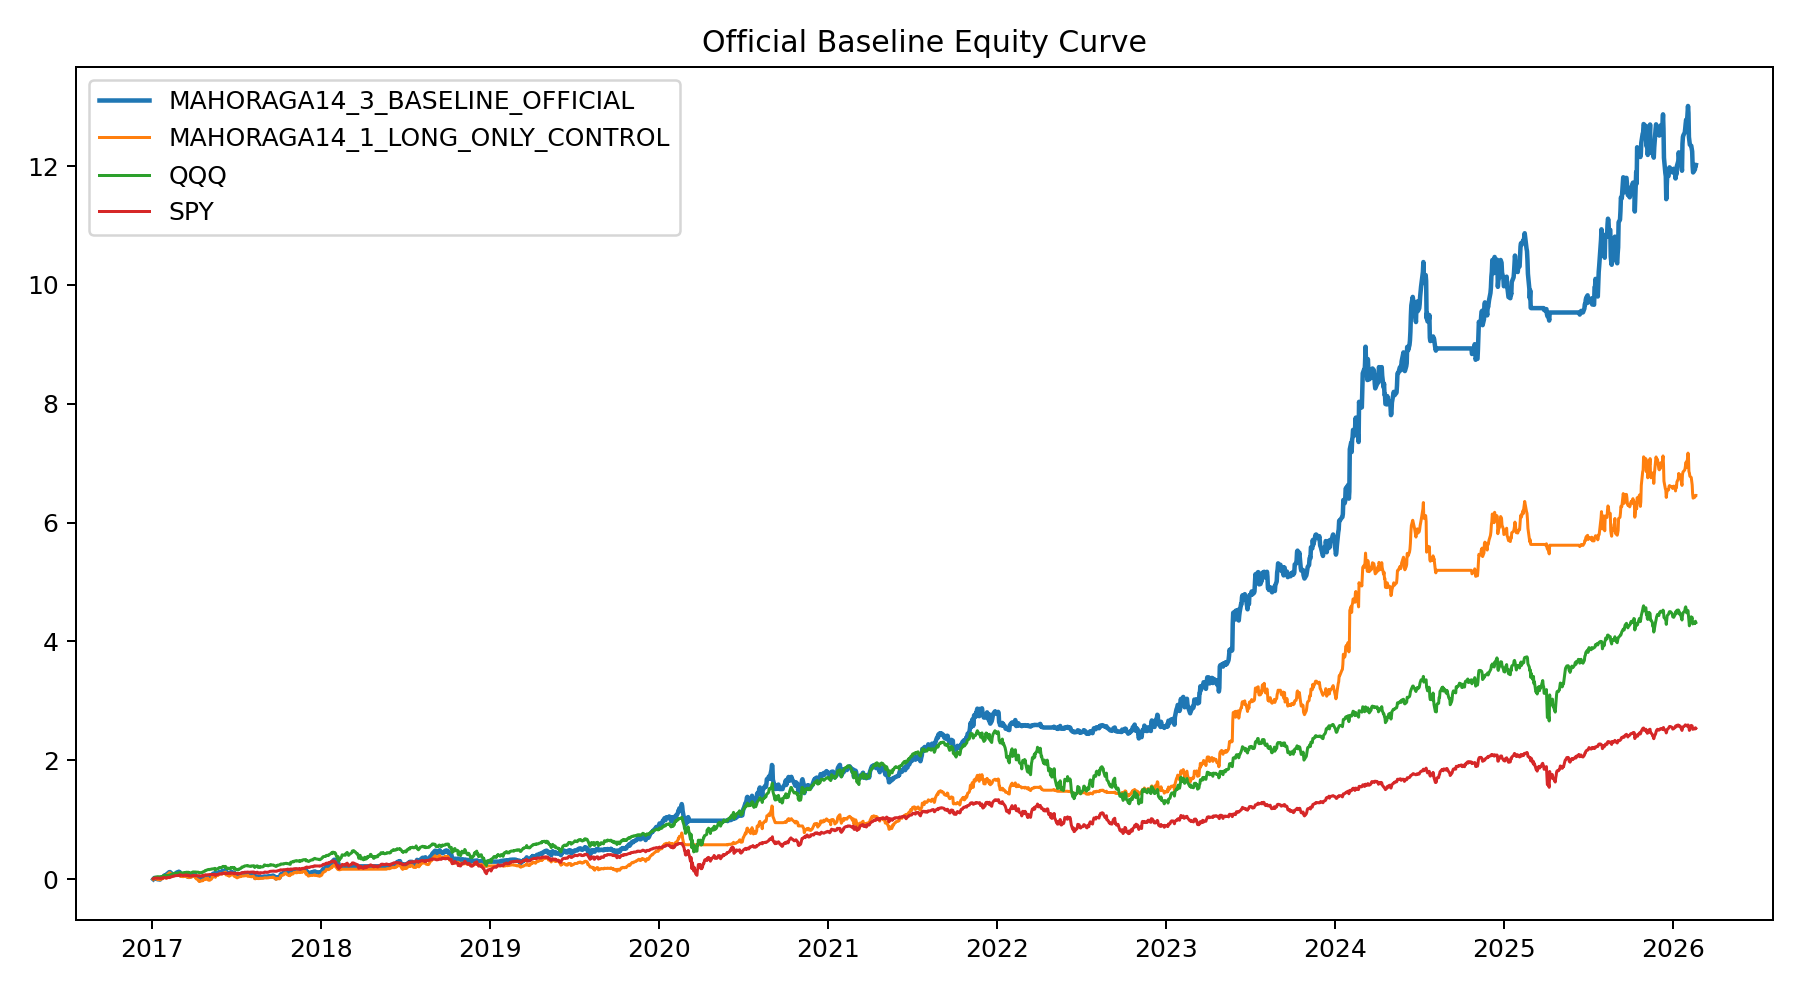
\includegraphics[width=\textwidth]{equity_curve_official.png}
\caption{Curva de equity oficial stitched del baseline publicado frente a referencias oficiales. La figura proviene de los outputs congelados del repositorio y debe interpretarse como resultado agregado OOS, no como prueba concluyente de estabilidad futura.}
\label{fig:equity}
\end{figure}

El resultado central es que el baseline promovido combina mayor CAGR y mejor perfil de drawdown que el control historico oficial en el stitched publicado. Sin embargo, la afirmacion metodologicamente correcta no es \enquote{ya se demostro superioridad absoluta}, sino \enquote{dentro del marco auditado del repositorio, el candidato promovido produce una mejora agregada con mejor robustez local que el control reemplazado}.

\subsection{Resultados por fold}
\begin{figure}[H]
\centering
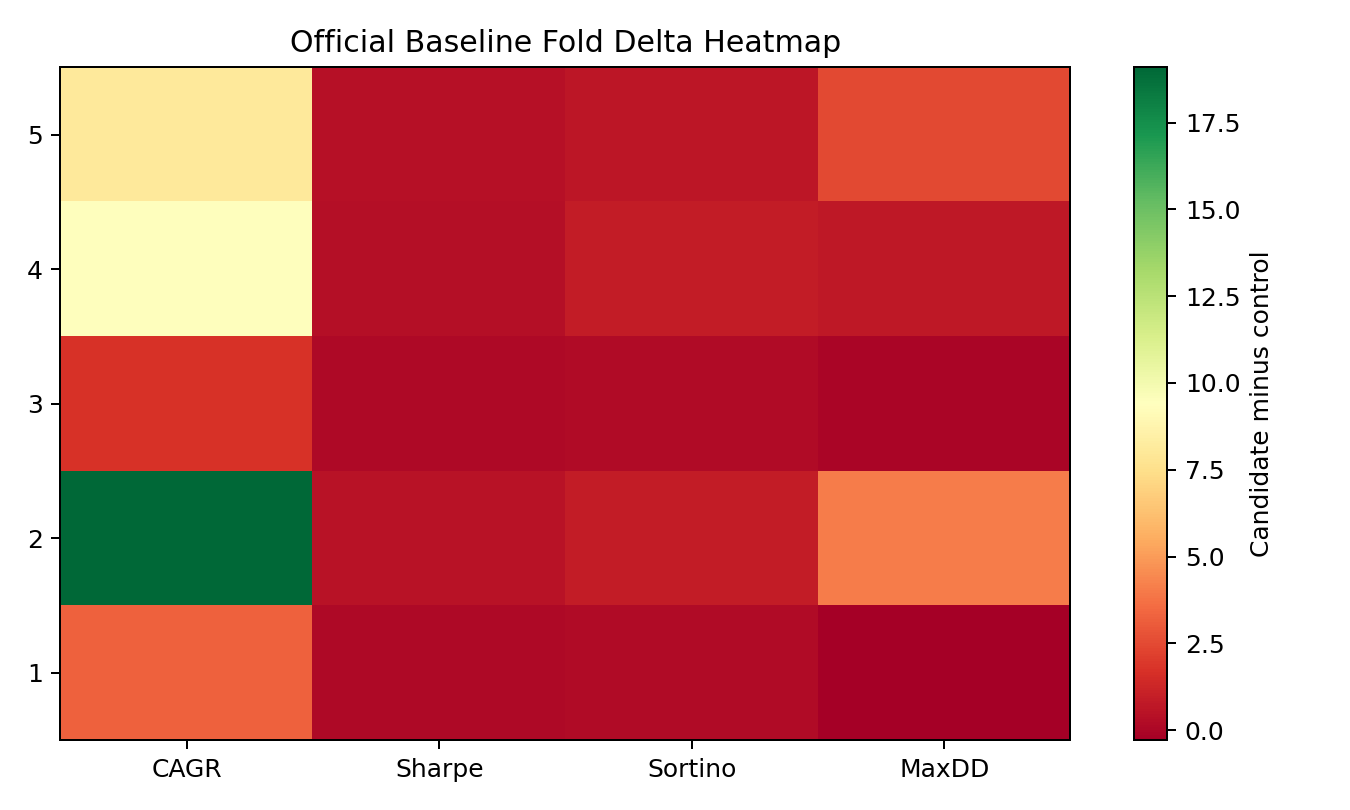
\includegraphics[width=\textwidth]{fold_heatmap_official.png}
\caption{Heatmap oficial por fold. Sirve para verificar que el comportamiento del candidato promovido no depende de un unico tramo del stitched.}
\label{fig:fold-heatmap}
\end{figure}

Los resultados por fold publicados muestran que el baseline oficial supera al control historico en CAGR en los cinco folds reportados. El tramo 2023-2024 es especialmente fuerte, pero no es el unico soporte: tambien hay mejora en 2017-2018, 2019-2020, 2021-2022 y 2024-2026.

\subsection{Ventanas prioritarias}
\begin{table}[H]
\centering
\caption{Ventanas prioritarias oficiales}
\label{tab:priority-windows}
\begin{tabularx}{\textwidth}{>{\raggedright\arraybackslash}p{0.16\textwidth}rrrrX}
\toprule
\textbf{Ventana} & \textbf{Candidate} & \textbf{Control} & \textbf{QQQ} & \textbf{SPY} & \textbf{Lectura} \\
\midrule
2017\_2018 & 0.2930 & 0.2213 & 0.3197 & 0.1614 & Pasa por mejora sobre control con calidad local aceptable. \\
2020\_2021 & 0.9074 & 0.6881 & 1.0997 & 0.8910 & Pasa por mantener mejora sobre control. \\
2023\_2024 & 2.0717 & 1.7480 & 0.9369 & 0.5758 & Pasa por conservar fortaleza bull reciente. \\
\bottomrule
\end{tabularx}
\end{table}

\begin{figure}[H]
\centering
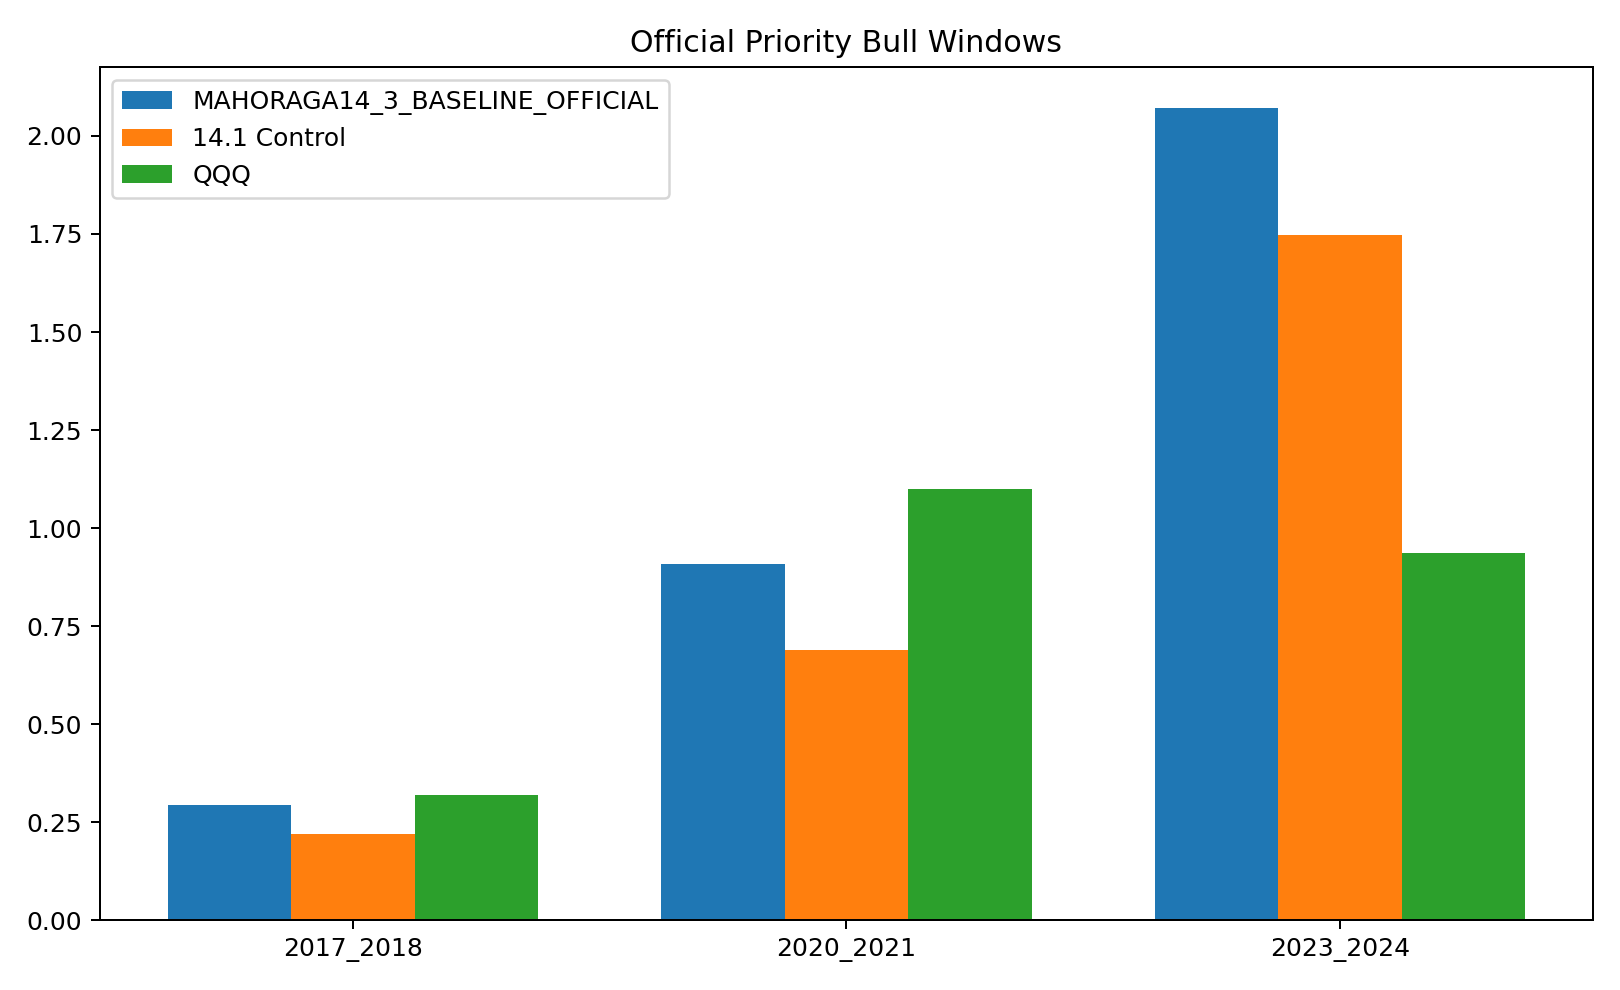
\includegraphics[width=\textwidth]{bull_window_scorecard_official.png}
\caption{Scorecard oficial de ventanas prioritarias. Estas ventanas son centrales para la decision institucional de promocion.}
\label{fig:bull-scorecard}
\end{figure}

\subsection{Alpha oficial frente a benchmarks}
\begin{table}[H]
\centering
\caption{Alpha Newey-West oficial}
\label{tab:alpha-nw}
\begin{adjustbox}{max width=\textwidth}
\begin{tabular}{p{0.28\textwidth}lrrrr}
\toprule
\textbf{Variante} & \textbf{Benchmark} & \textbf{Alpha ann} & \textbf{t(alpha)} & \textbf{p(alpha)} & \textbf{Beta} \\
\midrule
\historicalcontrol & QQQ & 0.149353 & 2.490 & 0.012777 & 0.4853 \\
\historicalcontrol & SPY & 0.182964 & 2.716 & 0.006617 & 0.4683 \\
\officiallabel & QQQ & 0.214661 & 3.613 & 0.000302 & 0.5159 \\
\officiallabel & SPY & 0.250536 & 3.739 & 0.000185 & 0.5077 \\
\bottomrule
\end{tabular}
\end{adjustbox}
\end{table}

Estos resultados sugieren que el baseline oficial no solo toma beta de mercado. Aun asi, una alpha lineal positiva no elimina todos los riesgos de especificacion: depende del benchmark elegido y de una descomposicion lineal concreta.

\subsection{P-values y q-values oficiales}
\begin{table}[H]
\centering
\caption{Pruebas oficiales de significancia comparativa}
\label{tab:pq}
\begin{adjustbox}{max width=\textwidth}
\begin{tabular}{p{0.24\textwidth}rrrrr}
\toprule
\textbf{Referencia} & \textbf{p-value} & \textbf{q-value} & \textbf{Delta CAGR} & \textbf{Delta Sharpe} & \textbf{Delta MaxDD} \\
\midrule
\historicalcontrol & 0.003170 & 0.017435 & 7.8676 & 0.2889 & 4.0355 \\
\code{QQQ} & 0.080356 & 0.147319 & 12.4106 & 0.5648 & 19.0419 \\
\code{SPY} & 0.014439 & 0.039708 & 17.6723 & 0.6363 & 17.5175 \\
\bottomrule
\end{tabular}
\end{adjustbox}
\end{table}

La mejora frente al control historico oficial es la comparacion institucionalmente mas importante, y ahi la evidencia estadistica reportada es mas fuerte que frente a \code{QQQ}. Esto es logico: el baseline no fue construido para \enquote{ganar siempre al benchmark Nasdaq en cualquier subtramo}, sino para reemplazar un control institucional previo con mejor robustez.

\subsection{Exposicion y eficiencia del despliegue}
\begin{table}[H]
\centering
\caption{Exposicion, turnover y eficiencia}
\label{tab:exposure-turnover}
\begin{adjustbox}{max width=\textwidth}
\begin{tabular}{p{0.34\textwidth}rrrr}
\toprule
\textbf{Variante} & \textbf{Avg exposure} & \textbf{Avg turnover} & \textbf{Return/exposure} & \textbf{Obs.} \\
\midrule
\officiallabel & 0.6534 & 0.0497 & 0.001838 & 2295 \\
\historicalcontrol & 0.6316 & 0.0345 & 0.001514 & 2295 \\
\bottomrule
\end{tabular}
\end{adjustbox}
\end{table}

El punto economico de esta tabla es sutil: el baseline oficial no solo gana mas en total, sino que gana mas por unidad media de capital desplegado. Eso apoya la lectura de que la capa de participacion no solo empuja exposicion, sino que la dosifica de forma mas eficiente.

\begin{figure}[H]
\centering
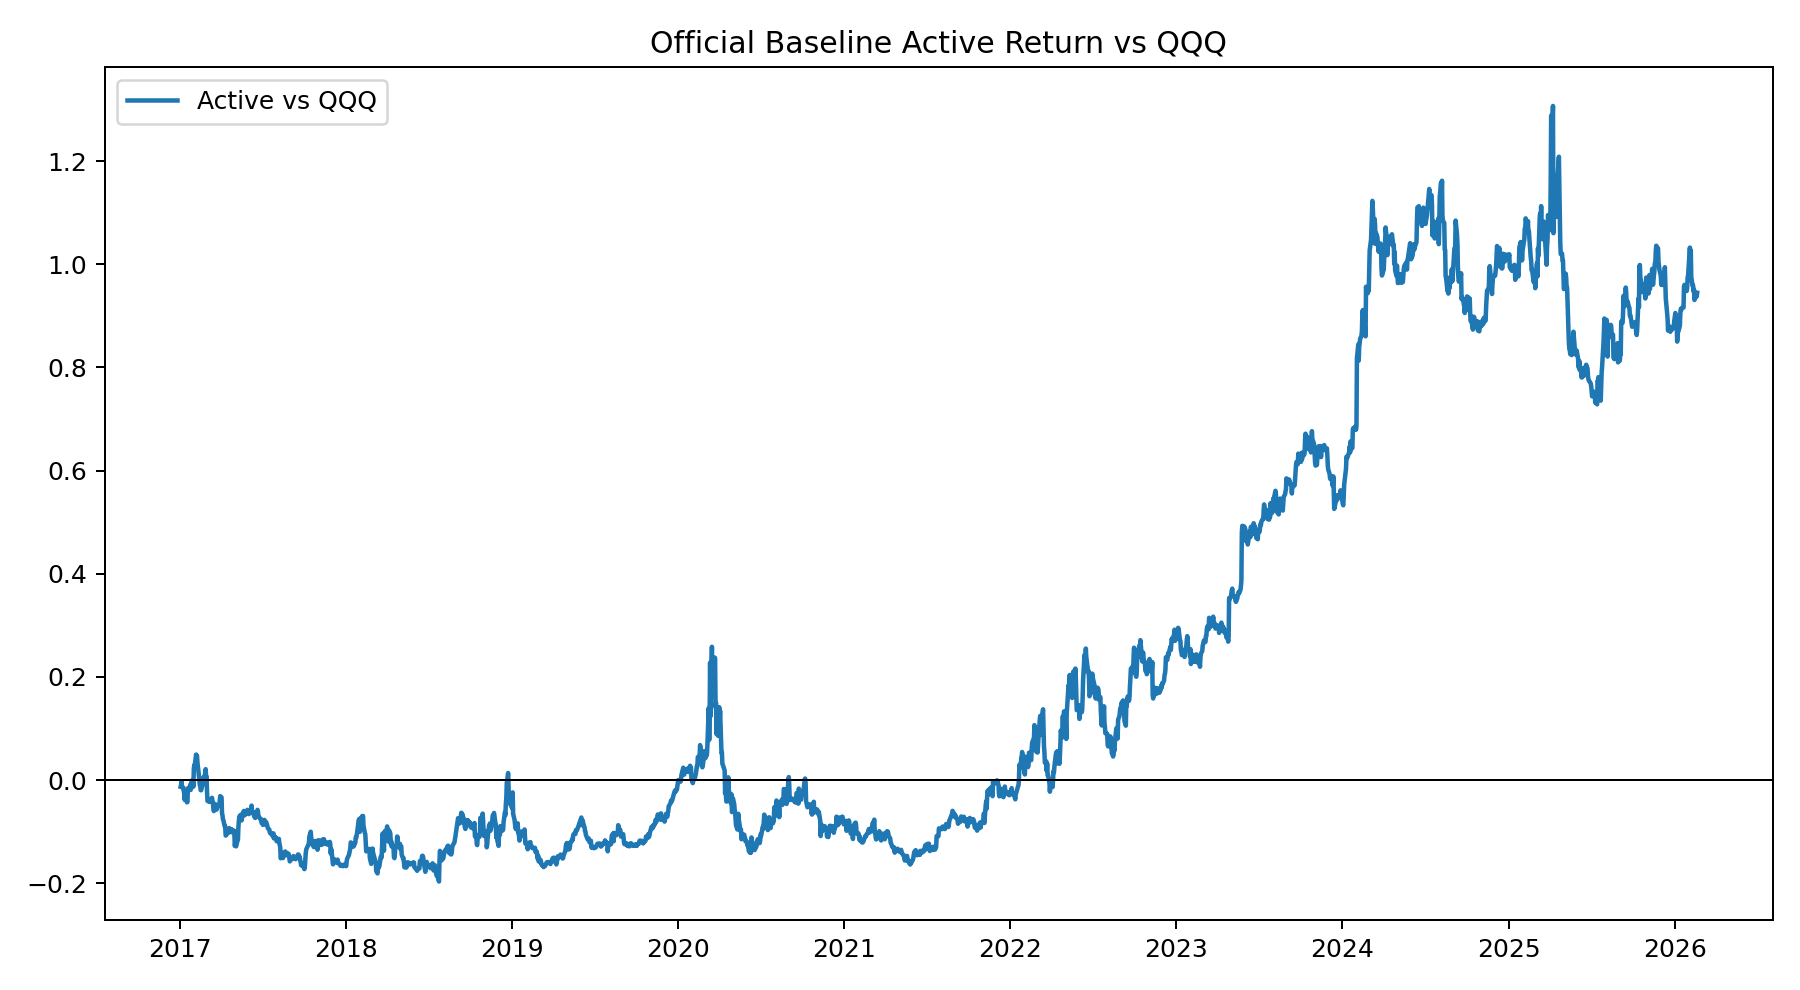
\includegraphics[width=\textwidth]{active_return_vs_qqq_official.png}
\caption{Retorno activo oficial frente a \code{QQQ}. Ayuda a distinguir periodos de aportacion y detraccion relativa del baseline.}
\label{fig:active-vs-qqq}
\end{figure}

\section{Robustez, estabilidad y riesgo de sobreajuste}
\subsection{Estabilidad local}
La auditoria de estabilidad local reporta:
\begin{itemize}
    \item candidato base-corriente: \code{B1.00\_C1.00\_L1.00\_R1.00}, robust score 0.5148;
    \item candidato oficial promovido: \officialcandidate, robust score 0.9951;
    \item \emph{plateau share} aceptado: 50.62\%.
\end{itemize}

\begin{figure}[H]
\centering
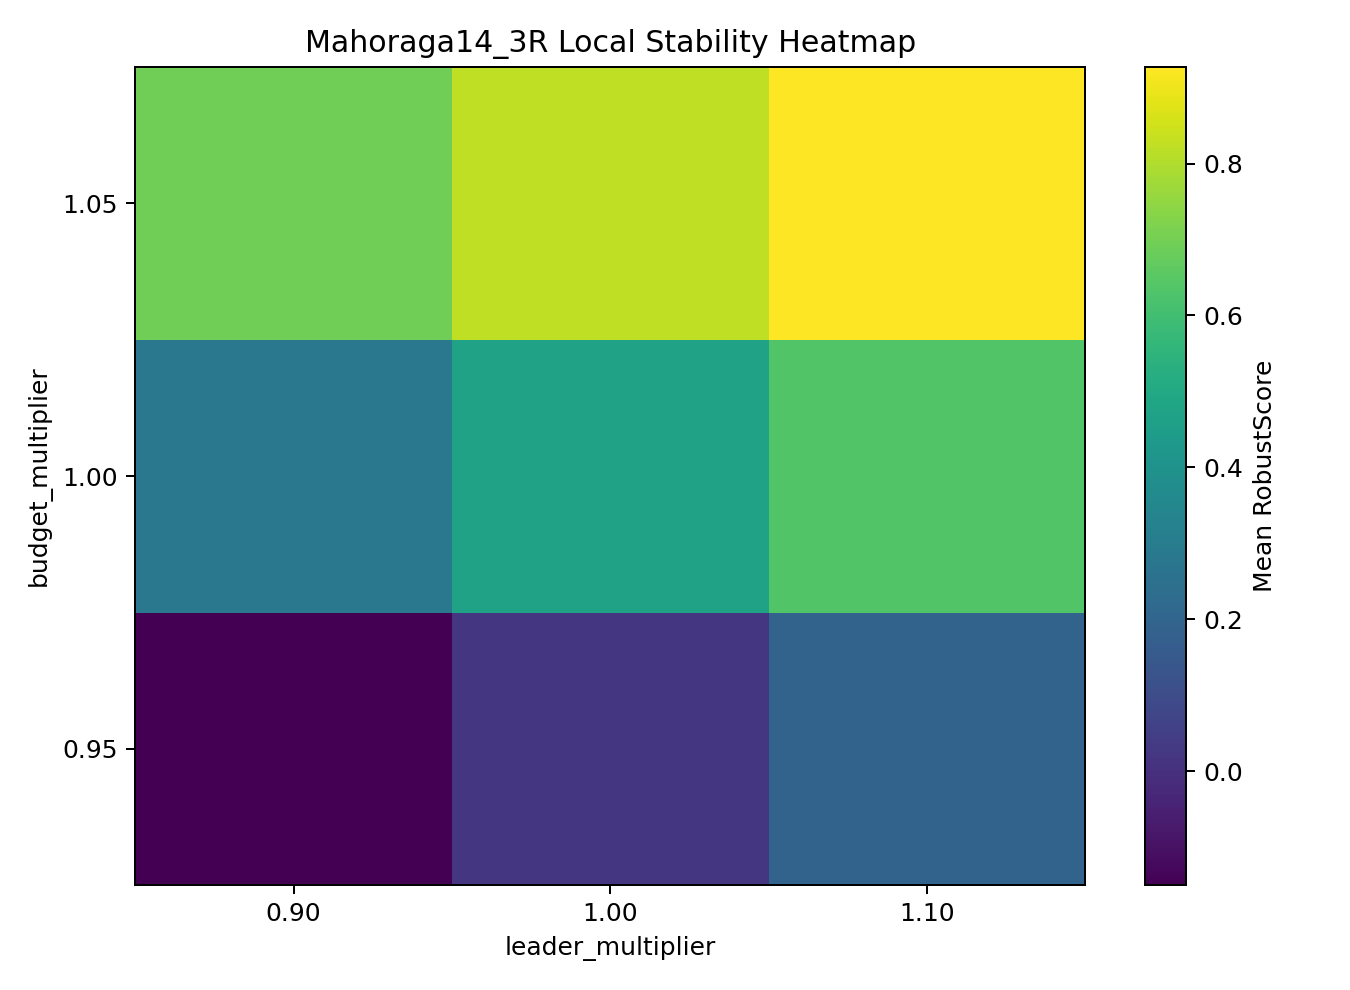
\includegraphics[width=\textwidth]{local_stability_heatmap_official.png}
\caption{Heatmap oficial de estabilidad local. La lectura institucional del repositorio es que el candidato promovido pertenece a una meseta robusta, no a un punto fragil aislado.}
\label{fig:local-stability}
\end{figure}

La interpretacion correcta es fuerte pero acotada: el candidato oficial parece robusto dentro de un vecindario local de su familia. No equivale a demostrar que sea optimo global en todo el espacio de estrategias posibles.

\subsection{Leave-one-window-out}
La prueba \emph{leave-one-window-out} excluye una ventana prioritaria por vez y repite la seleccion. El resultado oficial es que \officialcandidate{} es seleccionado en los tres experimentos de exclusion. Eso reduce la sospecha de que la promocion dependa de una sola ventana privilegiada.

\subsection{Bootstrap}
El bootstrap oficial por bloques estacionarios reporta medianas positivas:
\begin{itemize}
    \item \(\mathrm{DeltaCAGR}_{50} = 0.0792\);
    \item \(\mathrm{DeltaSharpe}_{50} = 0.2903\);
    \item \(\mathrm{DeltaMaxDD}_{50} = 0.0309\).
\end{itemize}

\begin{figure}[H]
\centering
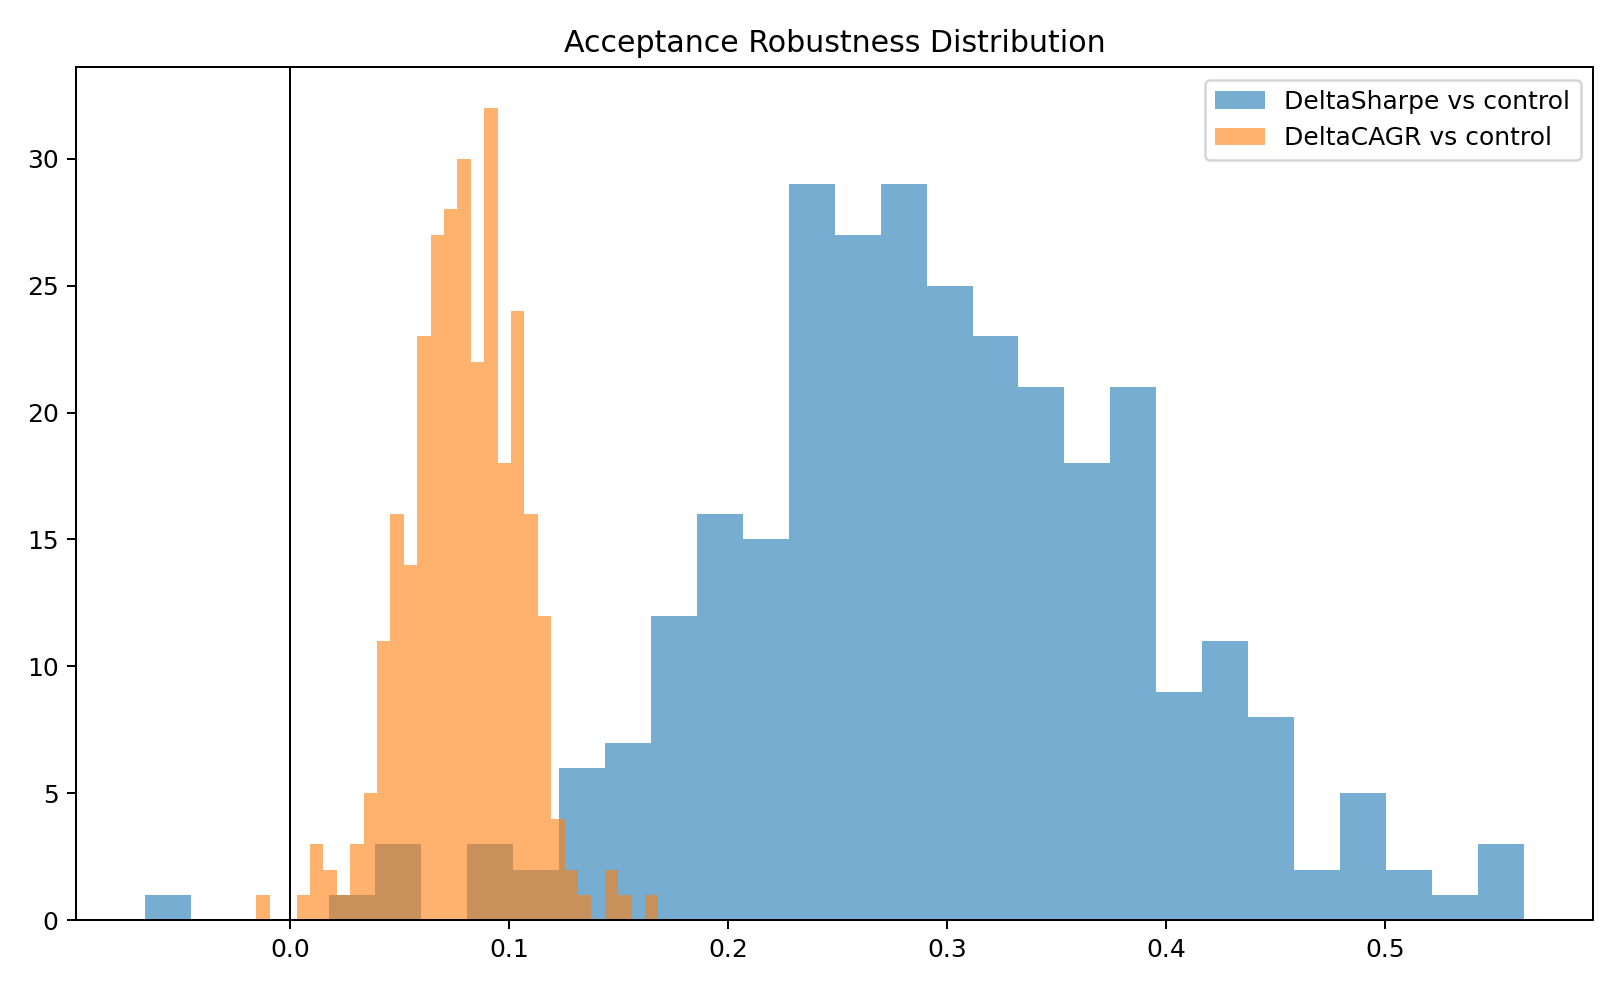
\includegraphics[width=\textwidth]{robustness_distribution_official.png}
\caption{Distribucion oficial de robustez bootstrap. Resume dispersion de desempeno del candidato promovido frente al control bajo re-muestreo temporal dependiente.}
\label{fig:bootstrap-robustness}
\end{figure}

\subsection{Model-selection guard}
La guarda de seleccion oficial informa:
\begin{itemize}
    \item \emph{local family reality-check p-value} = 0.0000;
    \item \emph{official candidate centered bootstrap p-value} = 0.0000.
\end{itemize}

El sentido practico de este artefacto es conservador. La familia 14.3R hereda iteraciones previas; por eso la promocion se defiende frente a \emph{data snooping} local, no se presenta ingenuamente como si hubiera existido un unico intento.

\subsection{Continuation como riesgo y como ayuda}
La auditoria de continuation es honesta. Reporta:
\begin{itemize}
    \item tasa de activacion stitched de 3.68\%;
    \item hit rate 4W de 58.33\%;
    \item hit rate 4W sin activacion de 55.63\%;
    \item edge de 4.58 puntos porcentuales.
\end{itemize}

La conclusion institucional es precisa: continuation ayuda, pero no justifica por si sola el baseline. Sirve mejor como filtro de calidad que como palanca principal de participacion.

\section{Fortalezas}
Las fortalezas mas defensibles del baseline oficial son las siguientes.

\begin{itemize}
    \item \textbf{Separacion de funciones.} El sistema diferencia entre seleccionar nombres y decidir intensidad de despliegue. Eso lo hace mas interpretable que un unico score opaco.
    \item \textbf{Arquitectura auditable.} Cada modulo tiene entradas y salidas conceptualmente claras, y existe documentacion institucional de freeze, promotion y audit trail.
    \item \textbf{Disciplina de control.} El baseline incluye stops, crisis gate, turbulence, corr shield, defense y backoff. No depende de una sola barrera de riesgo.
    \item \textbf{Robustez local documentada.} La promocion viene acompanada de plateau local, leave-one-window-out y bootstrap por bloques.
    \item \textbf{Economia de complejidad.} Aunque contiene ML, lo reserva para capas especificas y no lo usa para convertir todo el sistema en una caja negra.
    \item \textbf{Eficiencia de capital.} Los outputs oficiales sugieren mejor retorno por unidad de exposicion que el control institucional previo.
\end{itemize}

\section{Limitaciones}
El baseline oficial tambien tiene limitaciones importantes que no deben ocultarse.

\begin{itemize}
    \item \textbf{Universo pequeno y concentrado.} El sistema opera sobre un conjunto de nombres tecnologicos/liquidos relativamente reducido. Eso facilita interpretacion, pero expone a riesgo sectorial.
    \item \textbf{Long-only.} No hay sleeve corta ni hedge estructural. En ciertos mercados bajistas, la unica defensa es reducir exposicion, no ganar con la caida.
    \item \textbf{Dependencia de \code{QQQ}.} Benchmark, residualizacion y varias lecturas de estado descansan mucho en \code{QQQ}; esto puede limitar generalizacion a otros complejos.
    \item \textbf{Sensibilidad de capa sobre capa.} La arquitectura es interpretable, pero no trivial. Pequenos cambios pueden propagarse por score, stops, allocator, backoff y leader blend.
    \item \textbf{Riesgo residual de sobreajuste.} Hay protecciones serias, pero ninguna suite interna puede probar ausencia total de \emph{selection bias}.
    \item \textbf{Sin garantia de persistencia.} Que el stitched oficial sea fuerte no implica que el mismo perfil se mantenga fuera del periodo publicado.
    \item \textbf{Algunas ideas quedaron como inspiracion.} Eso es una virtud de honestidad, pero implica que el proyecto conceptual es mas amplio que la implementacion final efectivamente congelada.
\end{itemize}

\section{Posibles extensiones}
Las extensiones siguientes no deben confundirse con componentes ya implementados. Son direcciones razonables si se quisiera continuar la linea de trabajo sin romper la frontera entre baseline y research.

\begin{itemize}
    \item ampliar el universo y volver a auditar si la logica de participacion se sostiene fuera del complejo tecnologico concentrado;
    \item estudiar versiones multi-sleeve donde la parte long-only oficial conviva con sleeves defensivos separados y auditados;
    \item revisar si las features Hawkes-style agregan informacion incremental medible frente a versiones mas simples;
    \item reforzar pruebas de sensibilidad a ejecucion realista, gaps y liquidez;
    \item validar si la residualizacion frente a factores mas amplios o dinamicos mejora estabilidad sin introducir complejidad espuria;
    \item comparar la arquitectura con controles mas fuertes que el historico 14.1, siempre en regimen de gobernanza separado del baseline oficial.
\end{itemize}

\section{Conclusiones}
Mahoraga, en su baseline oficial congelado, debe entenderse como un sistema quant long-only de dos capas: un motor de seleccion de nombres basado en tendencia, momentum y residualizacion, y una capa de traduccion de contexto a participacion que decide cuanto capital desplegar, cuanto sesgo otorgar a lideres y cuando retroceder. Esa segunda capa es el rasgo que mas claramente distingue a la version 14.3R promovida del control historico que reemplaza.

El paper muestra que el baseline oficial no es una coleccion difusa de ideas. Tiene limites claros: no es un sistema long-short, no usa deep learning, no implementa Navier-Stokes, no usa un proceso Hawkes completo y no incluye como modulos oficiales varias exploraciones que existen en \code{research/}. A la vez, si incorpora ML real en zonas muy concretas y si incorpora una cadena extensa de control de riesgo y auditoria.

Los resultados oficiales stitched, por fold y por ventanas prioritarias favorecen al baseline promovido frente al control institucional previo. Pero la interpretacion correcta es metodologicamente sobria: la promocion se sostiene como mejora robusta dentro de una familia local aceptada y bajo una suite de auditorias seria, no como demostracion final de superioridad universal. Precisamente por eso el baseline puede servir como referencia institucional util: es suficientemente fuerte para operar como punto de partida oficial y suficientemente transparente para ser criticado, reconstruido y mejorado con disciplina.

\appendix

\section{Mapa del codigo fuente}
La \cref{tab:code-map} resume los archivos mas importantes para reconstruir el baseline.

\begin{longtable}{>{\raggedright\arraybackslash}p{0.24\textwidth}>{\raggedright\arraybackslash}p{0.12\textwidth}>{\raggedright\arraybackslash}p{0.22\textwidth}>{\raggedright\arraybackslash}p{0.30\textwidth}}
\caption{Mapa de archivos principales del baseline oficial}\label{tab:code-map}\\
\toprule
\textbf{Archivo} & \textbf{Oficial} & \textbf{Rol} & \textbf{Comentario} \\
\midrule
\endfirsthead
\toprule
\textbf{Archivo} & \textbf{Oficial} & \textbf{Rol} & \textbf{Comentario} \\
\midrule
\endhead
\code{official\_baseline\_runner.py} & Si & entrada principal & Ejecuta el baseline oficial congelado. \\
\code{official\_baseline\_suite.py} & Si & publicacion/auditoria & Genera outputs oficiales, acceptance summary, figuras y freeze artifacts. \\
\code{backtest\_executor.py} & Si & orquestacion & Coordina ejecucion de backtests y variantes. \\
\code{mahoraga14\_config.py} & Si & configuracion & Contiene knobs congelados, paths logicos y parametros base. \\
\code{mahoraga14\_data.py} & Si & datos & Descarga/carga OHLCV, benchmarks, VIX, factores y caches. \\
\code{mahoraga14\_universe.py} & Si & universo & Construye el universo PIT o fallback estatico. \\
\code{base\_alpha\_engine.py} & Si & stock selection & Genera el libro base de seleccion long-only. \\
\code{path\_structure\_features.py} & Si & features de trayectoria & Construye contexto de drawdown, eficiencia, breadth, correlacion, Hawkes-style y otros. \\
\code{continuation\_v2\_model.py} & Si & quality filter ML & Modelos de trigger, pressure y break-risk para continuation. \\
\code{structural\_defense\_model.py} & Si & defensa ML & Modela deterioro estructural del entorno. \\
\code{override\_policy.py} & Si & reglas de override & Decide structural defense vs continuation lift. \\
\code{participation\_allocator\_v2.py} & Si & budget/exposure & Traduce contexto a presupuesto, caps y leader blend. \\
\code{conviction\_amplifier\_layer.py} & Si & overlay alcista & Amplifica traduccion de conviccion en entornos sanos. \\
\code{leader\_participation\_layer.py} & Si & overlay de lideres & Sesga participacion hacia lideres y reduce cash drag. \\
\code{risk\_backoff\_layer\_v2.py} & Si & freno de riesgo & Recorta agresivamente cuando sube fragilidad. \\
\code{mahoraga6\_1.py} & Si, heredado & utilidades base & Aloja funciones heredadas de backtest, costos, stops, alpha y escalas base. \\
\code{transition\_recovery\_model.py} & Parcial & features Hawkes-style & Sus features se usan; sus clasificadores standalone no forman parte de la ruta oficial principal. \\
\code{acceptance\_suite\_14\_3R.py} & Si, soporte & acceptance research-to-freeze & Sirve para acceptance de la familia 14.3R. \\
\code{promotion\_gate\_suite.py} & Si, soporte & promotion gate & Consolida la promocion institucional previa al freeze. \\
\code{bull\_participation\_layer.py} & No en ruta final & historico & Pieza historica no declarada como modulo oficial del freeze final. \\
\code{participation\_allocator\_v1.py} & No en ruta final & historico & Version previa del allocator. \\
\code{risk\_backoff\_layer.py} & No en ruta final & historico & Version previa del backoff. \\
\code{mahoraga14\_2\_runner.py}, \code{mahoraga14\_3\_runner.py}, \code{mahoraga14\_3R\_runner.py} & Research/historia & linaje & Ayudan a reconstruir evolucion, pero no son la entrada oficial congelada. \\
\bottomrule
\end{longtable}

\section{Variables clave}
\begin{longtable}{>{\raggedright\arraybackslash}p{0.24\textwidth}>{\raggedright\arraybackslash}p{0.66\textwidth}}
\caption{Glosario de variables principales}\label{tab:variables}\\
\toprule
\textbf{Variable} & \textbf{Sentido operativo} \\
\midrule
\endfirsthead
\toprule
\textbf{Variable} & \textbf{Sentido operativo} \\
\midrule
\endhead
\code{base\_dd} & drawdown actual del libro base. \\
\code{base\_eff\_2w}, \code{base\_eff\_4w} & eficiencia del camino del libro base. \\
\code{stop\_density\_2w}, \code{stop\_density\_4w} & densidad reciente de stops, usada como senal de fragilidad. \\
\code{breadth\_63} & amplitud transversal reciente del universo. \\
\code{avg\_corr\_21} & correlacion media reciente entre miembros del universo. \\
\code{qqq\_ret\_2w}, \code{qqq\_rebound\_2w} & retorno y rebote recientes del benchmark principal. \\
\code{transition\_hawkes\_stress} & intensidad discreta de eventos de estres con decaimiento tipo Hawkes. \\
\code{transition\_hawkes\_recovery} & intensidad discreta de recuperacion con decaimiento tipo Hawkes. \\
\code{continuation\_trigger\_score} & score de activacion de continuation. \\
\code{continuation\_pressure\_score} & score de presion/continuidad alcista. \\
\code{continuation\_break\_risk\_p} & probabilidad estimada de ruptura del entorno continuation. \\
\code{structural\_p} & probabilidad estimada de deterioro estructural. \\
\code{fragility\_score} & score sintetico de fragilidad del entorno/libro. \\
\code{benchmark\_weakness\_score} & score de debilidad del benchmark. \\
\code{leader\_opportunity\_score} & oportunidad de inclinar participacion hacia lideres. \\
\code{cash\_drag\_pressure\_score} & presion para redeploy de caja. \\
\code{long\_budget\_raw} & presupuesto base de exposicion antes de backoff. \\
\code{leader\_blend\_raw} & intensidad de mezcla hacia libro de lideres. \\
\code{conviction\_multiplier\_raw} & multiplicador bruto de conviccion. \\
\code{participation\_state\_raw} & etiqueta de estado alcista/backoff previa a la capa final de riesgo. \\
\bottomrule
\end{longtable}

\section{Inventario minimo de outputs auditados}
\begin{longtable}{>{\raggedright\arraybackslash}p{0.32\textwidth}>{\raggedright\arraybackslash}p{0.22\textwidth}>{\raggedright\arraybackslash}p{0.36\textwidth}}
\caption{Artefactos auditados usados en este paper}\label{tab:artifacts}\\
\toprule
\textbf{Artefacto} & \textbf{Tipo} & \textbf{Uso en el paper} \\
\midrule
\endfirsthead
\toprule
\textbf{Artefacto} & \textbf{Tipo} & \textbf{Uso en el paper} \\
\midrule
\endhead
\code{outputs/stitched\_comparison\_official.csv} & tabla & resultados agregados stitched. \\
\code{outputs/fold\_summary\_official.csv} & tabla & resultados por fold. \\
\code{outputs/priority\_window\_acceptance\_official.csv} & tabla & ventanas prioritarias. \\
\code{outputs/alpha\_nw\_official.csv} & tabla & alpha y beta frente a QQQ/SPY. \\
\code{outputs/pvalue\_qvalue\_official.csv} & tabla & significancia y multiple testing. \\
\code{outputs/exposure\_summary\_official.csv} & tabla & exposicion media. \\
\code{outputs/turnover\_summary\_official.csv} & tabla & rotacion. \\
\code{outputs/return\_per\_exposure\_official.csv} & tabla & eficiencia de despliegue. \\
\code{outputs/cost\_sensitivity\_official.csv} & tabla & sensibilidad a costos. \\
\code{outputs/slippage\_sensitivity\_official.csv} & tabla & sensibilidad a slippage. \\
\code{audit/acceptance\_decision\_official.md} & memo & decision institucional y priority windows. \\
\code{audit/local\_stability\_summary\_official.md} & memo & robust score y plateau share. \\
\code{audit/leave\_one\_window\_out\_summary\_official.md} & memo & prueba de exclusion de ventanas. \\
\code{audit/model\_selection\_guard\_official.md} & memo & reality-check local y centered bootstrap. \\
\code{audit/bootstrap\_summary\_official.csv} & tabla & dispersion bootstrap. \\
\code{audit/continuation\_acceptance\_official.md} & memo & rol real de continuation. \\
\code{audit/continuation\_diagnostic\_official.csv} & tabla & tasas de activacion y hit rates. \\
\code{audit/upside\_participation\_decomposition\_official.csv} & tabla & descomposicion economica por ventanas bull. \\
\code{audit/leader\_miss\_analysis\_official.csv} & tabla & evidencia de lideres capturados o perdidos. \\
\code{audit/allocator\_cash\_drag\_official.csv} & tabla & trazas detalladas del allocator y despliegue de caja. \\
\bottomrule
\end{longtable}

\bibliographystyle{plainnat}
\bibliography{references}

\end{document}
